% NEXUS-GO: Master's dissertation defense, academic Beamer version.
% Hand-written (not generated from the HTML deck). Text and numbers follow docs/STORYLINE.md,
% which was audited against dissertation.tex; tables come from tables.tex (gen_tables.py).
% Build: latexmk -pdf nexus-go-academic.tex
\documentclass[aspectratio=169,10pt]{beamer}
\usepackage[T1]{fontenc}
\usepackage[utf8]{inputenc}
\usepackage{lmodern}
\usepackage{amsmath,amssymb}
\usepackage{booktabs}
\usepackage{appendixnumberbeamer}
\usepackage{tikz}
\usetikzlibrary{positioning,arrows.meta}
\graphicspath{{figures/}}

% ---- theme: sober, academic -------------------------------------------------
\usetheme{default}
\definecolor{ink}{HTML}{1B2A41}
\definecolor{accent}{HTML}{9B1B30}% Unicamp-like red, used sparingly
\definecolor{seq}{HTML}{2B6CB0}
\definecolor{net}{HTML}{C05621}
\definecolor{fus}{HTML}{2F855A}
\setbeamercolor{frametitle}{fg=ink}
\setbeamercolor{title}{fg=ink}
\setbeamercolor{structure}{fg=ink}
\setbeamercolor{alerted text}{fg=accent}
\setbeamercolor{footline}{fg=gray}
\setbeamerfont{frametitle}{series=\bfseries,size=\Large}
\setbeamertemplate{navigation symbols}{}
\setbeamertemplate{itemize items}[circle]
\setbeamertemplate{frametitle}{%
  \vspace*{0.6em}\insertframetitle\par\vspace{-0.35em}{\color{accent}\rule{\linewidth}{0.6pt}}}
\setbeamertemplate{footline}{%
  \leavevmode\hbox to\paperwidth{\hspace{1.2em}\scriptsize\usebeamercolor[fg]{footline}%
  Y.~Mauhnoom \,·\, NEXUS-GO\hfill\insertsectionhead\hfill\insertframenumber\,/\,\inserttotalframenumber\hspace{1.2em}}\vspace{0.6em}}
\setbeamertemplate{section in toc}[sections numbered]
\setbeamersize{text margin left=2.2em,text margin right=2.2em}

\newcommand{\src}[1]{\par\vfill\hfill{\scriptsize\color{gray}Dissertation: #1}}
\newcommand{\wF}{wF_{\max}}
\newcommand{\Smin}{S_{\min}}
\newcommand{\NX}[1]{\textsc{nexus-go}/#1}
% generated by gen_tables.py from data/thesis_tables.json; do not edit

% tab:cafa5
\newcommand{\TabCorpus}{%
\begin{tabular}{lrrrr}\toprule
Ontology & Training & Validation & Test & Terms \\ \midrule
Biological Process (BP) & 73,768 & 9,221 & 9,221 & {500} \\
Cellular Component (CC) & {74,328} & {9,292} & {9,292} & 498 \\
Molecular Function (MF) & 62,909 & 7,864 & 7,864 & 499 \\
\bottomrule\end{tabular}}

% tab:gnn_gcn_gat
\newcommand{\TabGNN}{%
\begin{tabular}{llrrrr}\toprule
Graph Encoder & Prediction Head & BP & CC & MF & AVG \\ \midrule
GCN (2 layers) & Vector & \textbf{55.78} & \textbf{66.35} & \textbf{67.83} & \textbf{63.32} \\
 & Vision & 53.10 & 63.33 & 65.46 & 60.63 \\
GAT (2 layers 4 heads) & Vector & 46.47 & 61.14 & 63.83 & 57.15 \\
 & Vision & 46.17 & 59.45 & 61.03 & 55.55 \\
\bottomrule\end{tabular}}

% tab:late_fusion
\newcommand{\TabLate}{%
\begin{tabular}{lrrrr}\toprule
Combination Rule & BP & CC & MF & AVG \\ \midrule
Linear interpolation ($\gamma$) & \textbf{57.96} & \textbf{68.79} & \textbf{74.44} & \textbf{67.06} \\
Maximum & 57.35 & 67.79 & 72.59 & 65.91 \\
Minimum & 56.38 & 68.09 & 72.69 & 65.72 \\
IC sigmoid & 57.03 & 67.57 & 73.88 & 66.16 \\
Degree sigmoid & 57.02 & 67.76 & 72.42 & 65.73 \\
Master equation & 57.42 & 68.10 & 73.93 & 66.48 \\
Stacking (decision tree) & 56.22 & 67.35 & 73.76 & 65.78 \\
Stacking (logistic regression) & 57.53 & 68.50 & 72.47 & 66.17 \\
Stacking (MLP) & 56.92 & 68.12 & 73.92 & 66.32 \\
Stacking (random forest) & 56.65 & 68.21 & 74.14 & 66.33 \\
Stacking (gradient boosting) & 56.67 & 67.72 & 74.18 & 66.19 \\
\bottomrule\end{tabular}}

% tab:vetor_visao_ontologia
\newcommand{\TabVV}{%
\begin{tabular}{llrrrr}\toprule
Stage & Prediction Head & BP & CC & MF & AVG \\ \midrule
First Generation & Vector & 36.37 & 48.25 & 48.92 & 44.51 \\
 & Vision & 30.40 & 40.84 & 42.42 & 37.89 \\
Fixed propagation & Vector & 55.23 & 66.94 & 73.18 & 65.12 \\
 & Vision & 52.17 & 63.06 & 68.25 & 61.16 \\
End-to-end GNN & Vector & 55.78 & 66.35 & 67.83 & 63.32 \\
 & Vision & 53.10 & 63.33 & 65.46 & 60.63 \\
Early fusion & Vector & {56.52} & {67.20} & {73.81} & {65.84} \\
 & Vision & 53.17 & 64.77 & 69.52 & 62.49 \\
\bottomrule\end{tabular}}

% tab:confronto_bp
\newcommand{\TabTestBP}{%
\begin{tabular}{lrrrrrr}\toprule
Method & $F_{\max}$ & $F^{*}_{\max}$ & $wF_{\max}$ & AuPRC & IAuPRC & $S_{\min}\downarrow$ \\ \midrule
Naive baseline & 44.26 & 42.23 & 40.22 & 40.42 & 37.28 & 22.28 \\
DeepGraphGO & 55.29 & 52.21 & 48.92 & 54.04 & 57.89 & 20.11 \\
SEGT-GO & 52.05 & 48.22 & 44.57 & 42.82 & 50.71 & 21.24 \\
Mashup & 43.58 & 41.86 & 39.64 & 34.82 & 32.57 & 23.22 \\
MELISSA & 41.94 & 40.08 & 37.72 & 32.72 & 31.17 & 23.42 \\
deepNF & 35.59 & 31.14 & 26.95 & 34.15 & 33.66 & 25.73 \\ \midrule
First Generation & 46.25 & 39.86 & 37.30 & 45.57 & 47.37 & 23.68 \\
ProtT5 baseline & 59.61 & 56.31 & 53.74 & 58.53 & 62.92 & 18.92 \\ \midrule
NEXUS-GO/Fixed & 61.27 & 58.13 & 55.61 & 60.39 & 65.09 & 18.30 \\
NEXUS-GO/GNN & 62.05 & 59.17 & 56.95 & 60.97 & 66.27 & 17.66 \\
NEXUS-GO/Early & 62.87 & 59.81 & 57.51 & 62.42 & 65.73 & 17.35 \\
NEXUS-GO/Late & \textbf{63.74} & \textbf{60.96} & \textbf{58.69} & \textbf{64.02} & \textbf{68.83} & \textbf{17.12} \\
\bottomrule\end{tabular}}

% tab:confronto_cc
\newcommand{\TabTestCC}{%
\begin{tabular}{lrrrrrr}\toprule
Method & $F_{\max}$ & $F^{*}_{\max}$ & $wF_{\max}$ & AuPRC & IAuPRC & $S_{\min}\downarrow$ \\ \midrule
Naive baseline & 58.43 & 56.52 & 48.13 & 56.26 & 51.22 & 10.84 \\
DeepGraphGO & 73.74 & 71.11 & 60.35 & 71.88 & 78.59 & 9.67 \\
SEGT-GO & 71.18 & 68.07 & 55.52 & 63.24 & 74.74 & 10.42 \\
Mashup & 59.37 & 57.44 & 48.28 & 51.27 & 50.30 & 11.06 \\
MELISSA & 58.54 & 56.51 & 47.19 & 49.78 & 48.97 & 11.23 \\
deepNF & 62.49 & 57.59 & 36.51 & 58.44 & 65.10 & 13.52 \\ \midrule
First Generation & 67.38 & 63.46 & 48.39 & 63.83 & 72.20 & 12.03 \\
ProtT5 baseline & 76.79 & 74.29 & 64.78 & 73.30 & 82.06 & 9.47 \\ \midrule
NEXUS-GO/Fixed & 78.20 & 75.85 & 66.93 & 74.32 & 83.78 & 8.85 \\
NEXUS-GO/GNN & 78.42 & 76.01 & 66.70 & 74.41 & 84.07 & 8.44 \\
NEXUS-GO/Early & 78.42 & 76.02 & 67.18 & 74.33 & 83.72 & 8.57 \\
NEXUS-GO/Late & \textbf{79.72} & \textbf{77.52} & \textbf{69.02} & \textbf{76.73} & \textbf{86.26} & \textbf{8.22} \\
\bottomrule\end{tabular}}

% tab:confronto_mf
\newcommand{\TabTestMF}{%
\begin{tabular}{lrrrrrr}\toprule
Method & $F_{\max}$ & $F^{*}_{\max}$ & $wF_{\max}$ & AuPRC & IAuPRC & $S_{\min}\downarrow$ \\ \midrule
Naive baseline & 52.54 & 48.26 & 43.38 & 49.41 & 45.93 & 8.46 \\
DeepGraphGO & 76.98 & 73.14 & 68.96 & 74.03 & 80.41 & 5.67 \\
SEGT-GO & 73.40 & 68.76 & 64.12 & 58.64 & 75.15 & 6.37 \\
Mashup & 54.52 & 49.82 & 44.22 & 47.87 & 47.29 & 8.30 \\
MELISSA & 53.57 & 48.65 & 42.86 & 46.43 & 46.31 & 8.47 \\
deepNF & 58.43 & 48.70 & 39.00 & 54.55 & 53.49 & 9.36 \\ \midrule
First Generation & 61.04 & 53.38 & 48.62 & 49.34 & 62.42 & 9.20 \\
ProtT5 baseline & 79.75 & 76.02 & 72.57 & 73.75 & 82.25 & 5.31 \\ \midrule
NEXUS-GO/Fixed & 79.75 & 76.02 & 72.57 & 73.75 & 82.25 & 5.31 \\
NEXUS-GO/GNN & 76.09 & 71.74 & 67.77 & 67.50 & 80.64 & 6.04 \\
NEXUS-GO/Early & 80.22 & 76.54 & 72.94 & \textbf{81.88} & 82.05 & 5.22 \\
NEXUS-GO/Late & \textbf{80.89} & \textbf{77.41} & \textbf{73.89} & 76.53 & \textbf{84.92} & \textbf{5.14} \\
\bottomrule\end{tabular}}

% tab:custo
\newcommand{\TabCost}{%
\begin{tabular}{lrrrrrr}\toprule
Family & Runs & s/epoch & h/run & Total h & VRAM (GiB) & Epochs \\ \midrule
Fixed propagation + vector head & 49 & \textbf{5.24} & 0.35 & 15.1 & \textbf{6.4} & 250 \\
Fixed propagation + vision head & 26 & 18.45 & 0.17 & 4.5 & \textbf{6.4} & 35 \\
End-to-end GNN + vector head & 6 & 102.14 & 6.09 & 38.7 & 20.7 & 213 \\
End-to-end GNN + vision head & 6 & 108.41 & 4.35 & 31.3 & 21.1 & 138 \\
Early fusion + vector head & 40 & 5.26 & 0.27 & 10.2 & \textbf{6.4} & 205 \\
Early fusion + vision head & 20 & 18.63 & \textbf{0.16} & 3.2 & \textbf{6.4} & 30 \\
\bottomrule\end{tabular}}

% tab:degree_graph_gain
\newcommand{\TabGain}{%
\begin{tabular}{lrrr}\toprule
Degree Band & BP & CC & MF \\ \midrule
0 (isolated) & +3.24 [h] & +1.66 [f] & +0.21 [h] \\
1--2 & +1.68 [h] & +2.18 [f] & +0.24 [h] \\
3--5 & +1.77 [f] & +2.31 [f] & $-$0.33 [h] \\
6--14 & +3.79 [h] & +2.44 [h] & +1.06 [h] \\
15--49 & +5.97 [h] & +4.01 [g] & +1.73 [h] \\
$\geq$ 50 & +9.05 [h] & +8.71 [g] & +4.64 [h] \\
\bottomrule\end{tabular}}

% tab:cobertura
\newcommand{\TabCov}{%
\begin{tabular}{lrrr}\toprule
Method family & BP (\%) & CC (\%) & MF (\%) \\ \midrule
DeepGraphGO / SEGT-GO & 96.3 & 95.1 & 95.7 \\
Mashup / MELISSA / deepNF & 63.6 & 66.6 & 68.7 \\
This work (all routes) & 100.0 & 100.0 & 100.0 \\
\bottomrule\end{tabular}}


\title{NEXUS-GO}
\subtitle{Network-Extended Unified Sequence Embeddings\\for Gene Ontology Function Annotation}
\author{Yeonatan Mauhnoom}
\institute{Advisor: Prof.\ Dr.\ Zanoni Dias\\
  Co-advisors: Prof.\ Dr.\ Hélio Pedrini and Dr.\ Gabriel Bianchin de Oliveira\\[0.6em]
  Master's dissertation defense\\Institute of Computing, University of Campinas (Unicamp)}
\date{November 16, 2026}
\hypersetup{pdftitle={NEXUS-GO: Master's dissertation defense}, pdfauthor={Yeonatan Mauhnoom}}

\begin{document}

% ============================================================================ Opening
\begin{frame}[plain]
  \titlepage
\end{frame}

\begin{frame}{Roadmap}
  \begin{enumerate}
    \item Motivation: the sequence-function gap
    \item Background and related work
    \item Data and evaluation
    \item Method: two generations, four NEXUS-GO routes
    \item Results: ablations, literature, cost, connectivity
    \item Conclusions
  \end{enumerate}
  \vspace{1em}
  Every model is described by the same three decisions:\\
  \textbf{representation} $\rightarrow$ \textbf{propagation} $\rightarrow$ \textbf{prediction head}
  \src{Chapter 1, Document Structure}
\end{frame}

% ============================================================================ Motivation
\section{Motivation}

\begin{frame}{Millions of sequences, few known functions}
  \begin{itemize}[<+->]
    \item Proteins take part in almost every cellular process
    \item Sequencing is fast; experimental characterization is slow and expensive
    \item Few records carry experimentally supported annotations
    \item Automated prediction tries to close the gap (CAFA benchmark)
  \end{itemize}
  \src{§1.1; §3.1.1}
\end{frame}

\begin{frame}{Function as a hierarchy of terms}
  \begin{columns}[T]
    \column{0.42\textwidth}
    \begin{itemize}
      \item Three ontologies: Biological Process (BP), Cellular Component (CC), Molecular Function (MF)
      \item Each is a directed acyclic graph of terms (\texttt{is\_a}, \texttt{part\_of})
      \item \alert{True Path Rule}: a term implies all its ancestors
      \item Task: hierarchical multi-label classification
    \end{itemize}
    \column{0.56\textwidth}
    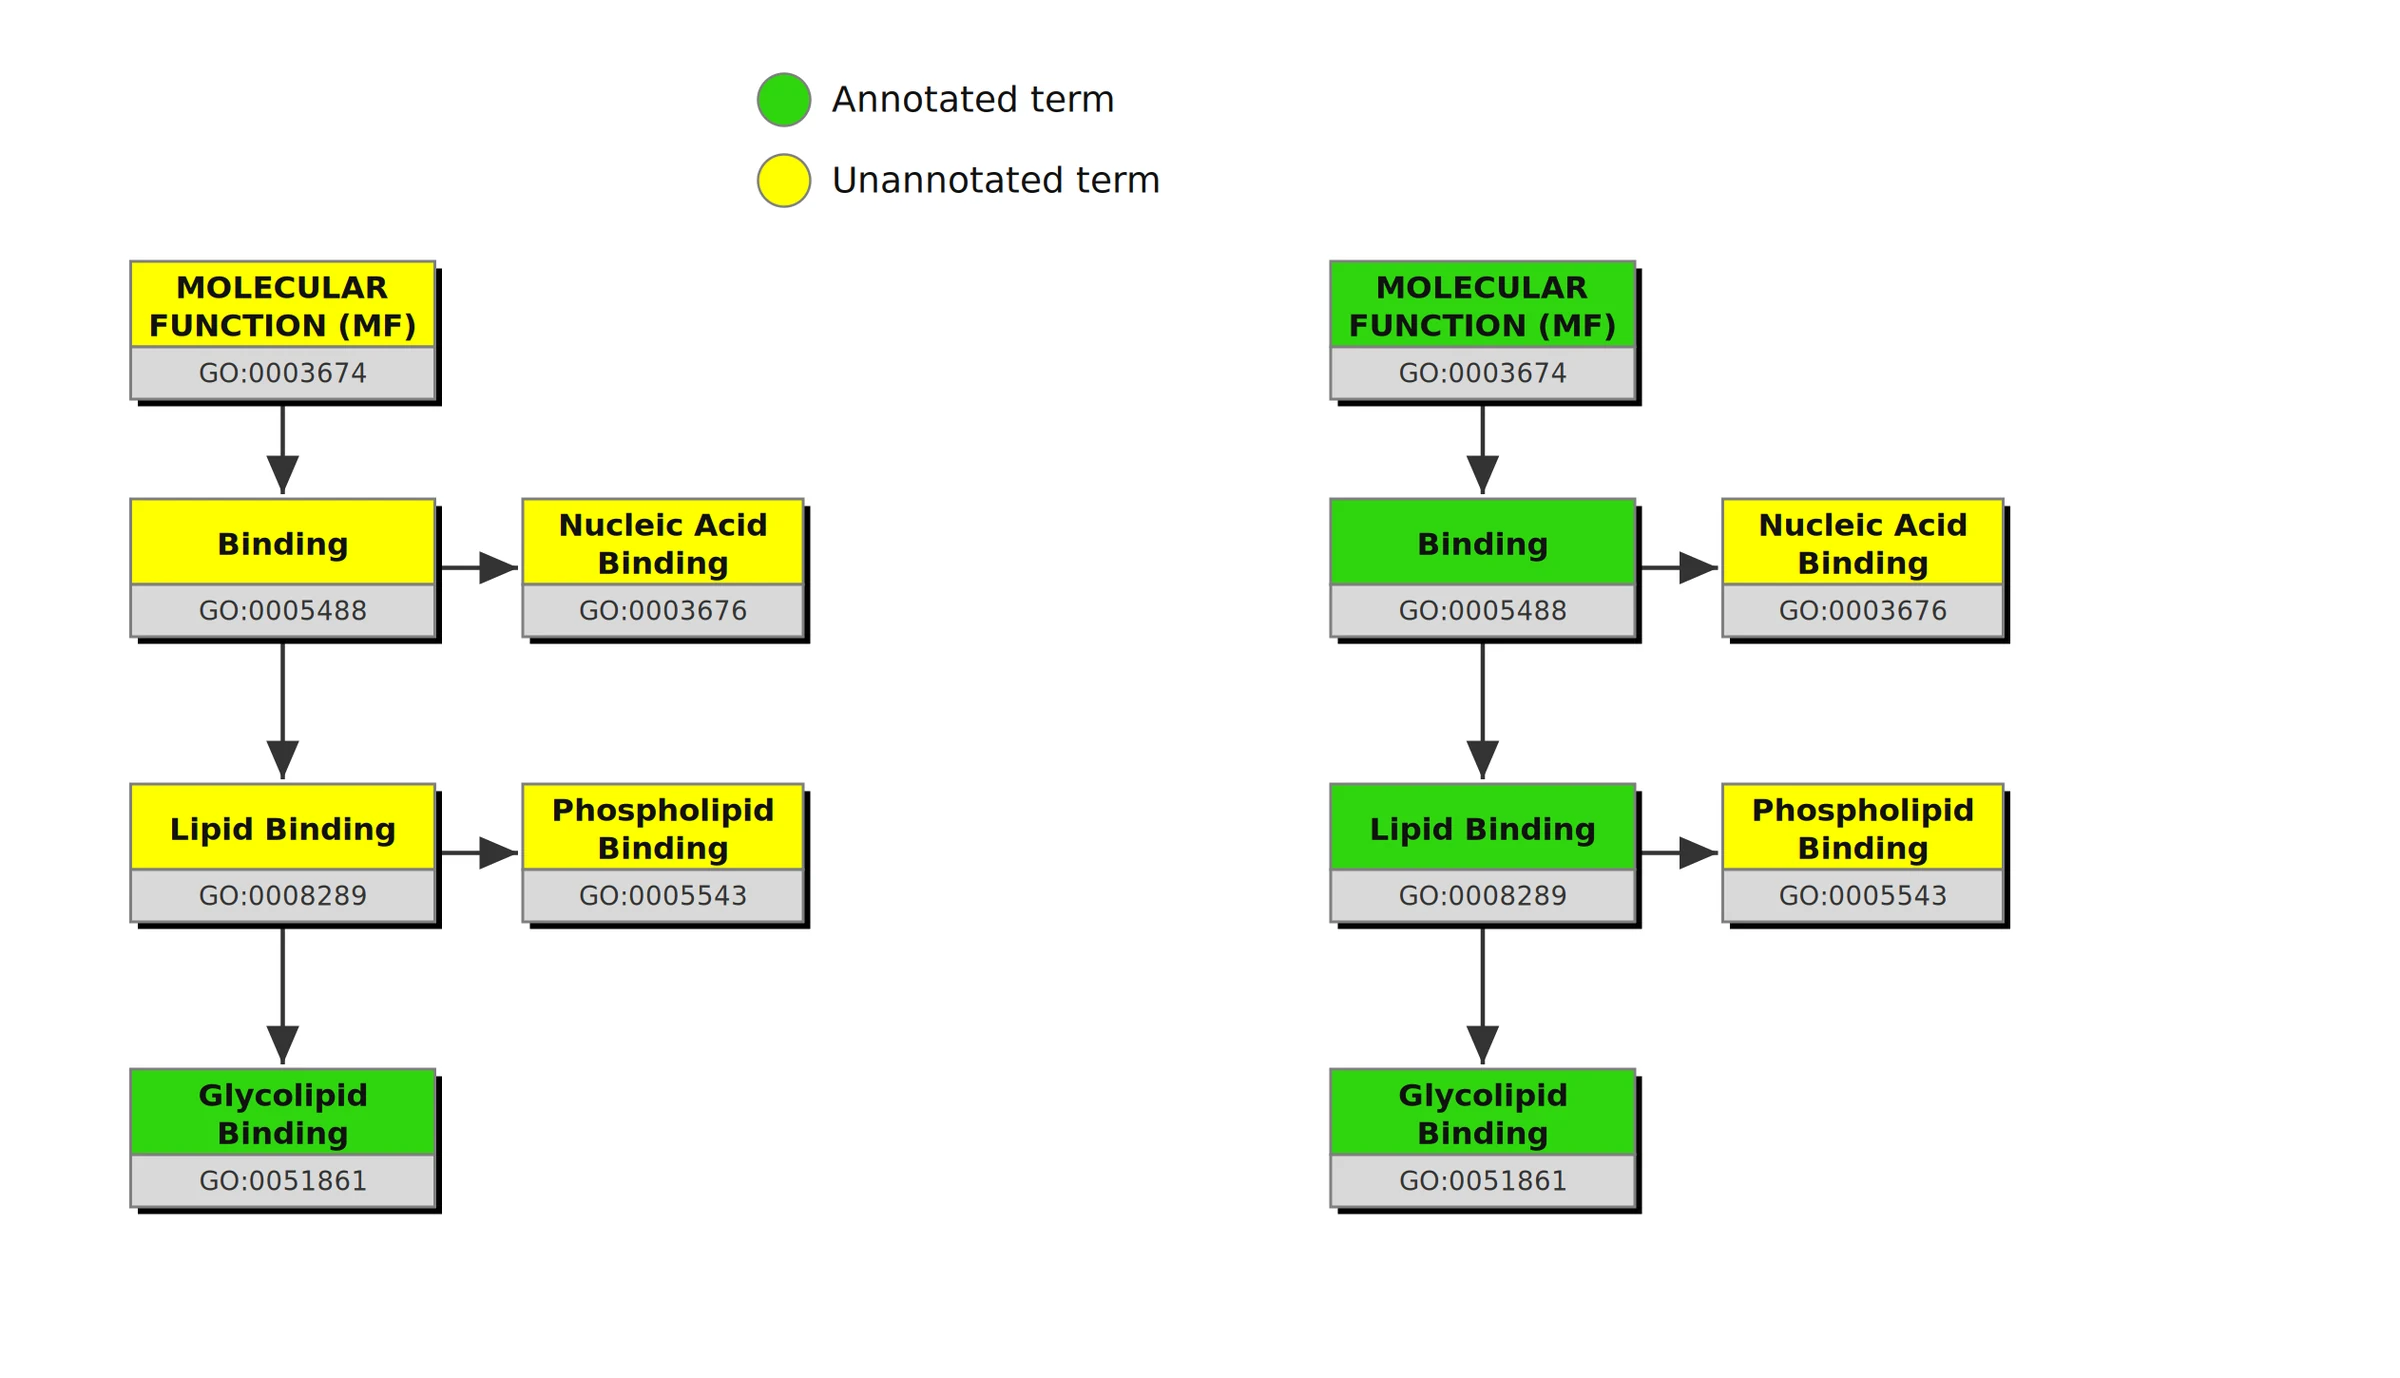
\includegraphics[width=\linewidth]{fig_2_1}\\
    {\scriptsize Fig.~2.1: inconsistent (left) and consistent (right) annotation.}
  \end{columns}
  \src{§2.1.2; §4.2, Eq.~4.1}
\end{frame}

\begin{frame}{Function also depends on context}
  \begin{columns}[T]
    \column{0.6\textwidth}
    \begin{itemize}
      \item Proteins act in complexes and pathways
      \item PPI networks: nodes are proteins, edges are associations
      \item Guilt by association: connected proteins tend to share functions
      \item<2-> \alert{But} STRING mixes evidence of uneven reliability, and about one third of proteins have no edge
    \end{itemize}
    \column{0.36\textwidth}
    \centering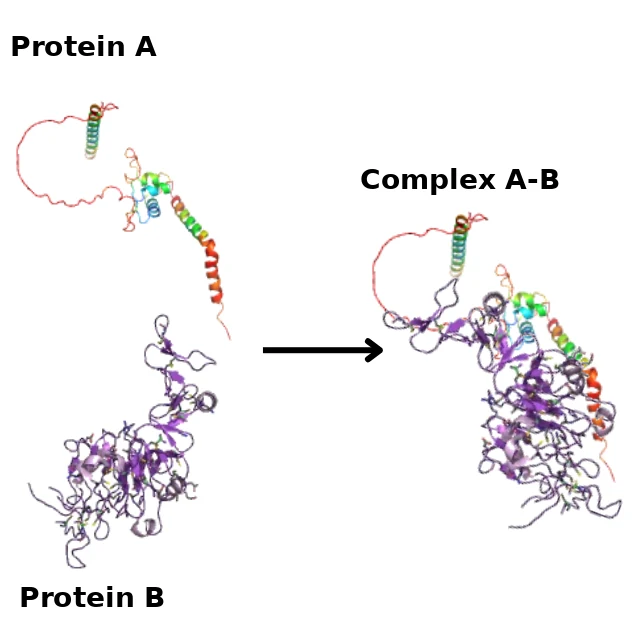
\includegraphics[width=0.85\linewidth]{fig_2_2}\\
    {\scriptsize Fig.~2.2: a protein complex.}
  \end{columns}
  \src{§1.1; §2.1.3; §4.1.3}
\end{frame}

\begin{frame}{Seven research questions}
  \begin{description}[RQ7]
    \item[RQ1] Which network representation works best?
    \item[RQ2] How much does propagating ProtT5 over STRING add?
    \item[RQ3] Fixed vs learned aggregation, vector vs image heads
    \item[RQ4] Do early and late fusion help?
    \item[RQ5] How deep, and how much retention?
    \item[RQ6] How does it compare with the literature?
    \item[RQ7] Does it work on one global, aggregated network?
  \end{description}
  \src{§1.3}
\end{frame}

\begin{frame}{Contributions}
  \begin{enumerate}
    \item NEXUS-GO: non-parametric multi-hop propagation of ProtT5 embeddings over STRING
    \item Controlled comparison of fixed vs learned (GCN, GAT) aggregation
    \item Vector vs image classification heads over the same embeddings
    \item Early and late fusion of fixed and learned routes
    \item Benchmark against five reimplemented methods, same splits and setting
  \end{enumerate}
  \vspace{0.6em}
  \textbf{Publications}\\[0.2em]
  {\small
  VISAPP 2026: \emph{From Graphs to Images: Non-Parametric PPI Context Integration for Vision-Based Protein Function Prediction}, pp.~157--166.\\[0.2em]
  Extended version: \emph{Beyond Learnable Graphs: Fixed Multi-Hop PPI Diffusion of Sequence Embeddings for Robust Protein Function Prediction}, accepted in CCIS (expected December 2026).}
  \src{§1.4; §1.5}
\end{frame}

% ============================================================================ Background
\section{Background and related work}

\begin{frame}{Graphs, adjacency and message passing}
  \begin{columns}[T]
    \column{0.45\textwidth}
    \begin{itemize}
      \item $G=(V,E,w)$: proteins, associations, STRING confidence
      \item Adjacency matrix $A$; sparse storage $O(|E|)$
      \item Message passing: aggregate neighbours, update the node
      \item $L$ layers reach $L$ hops; too many cause oversmoothing
    \end{itemize}
    \column{0.53\textwidth}
    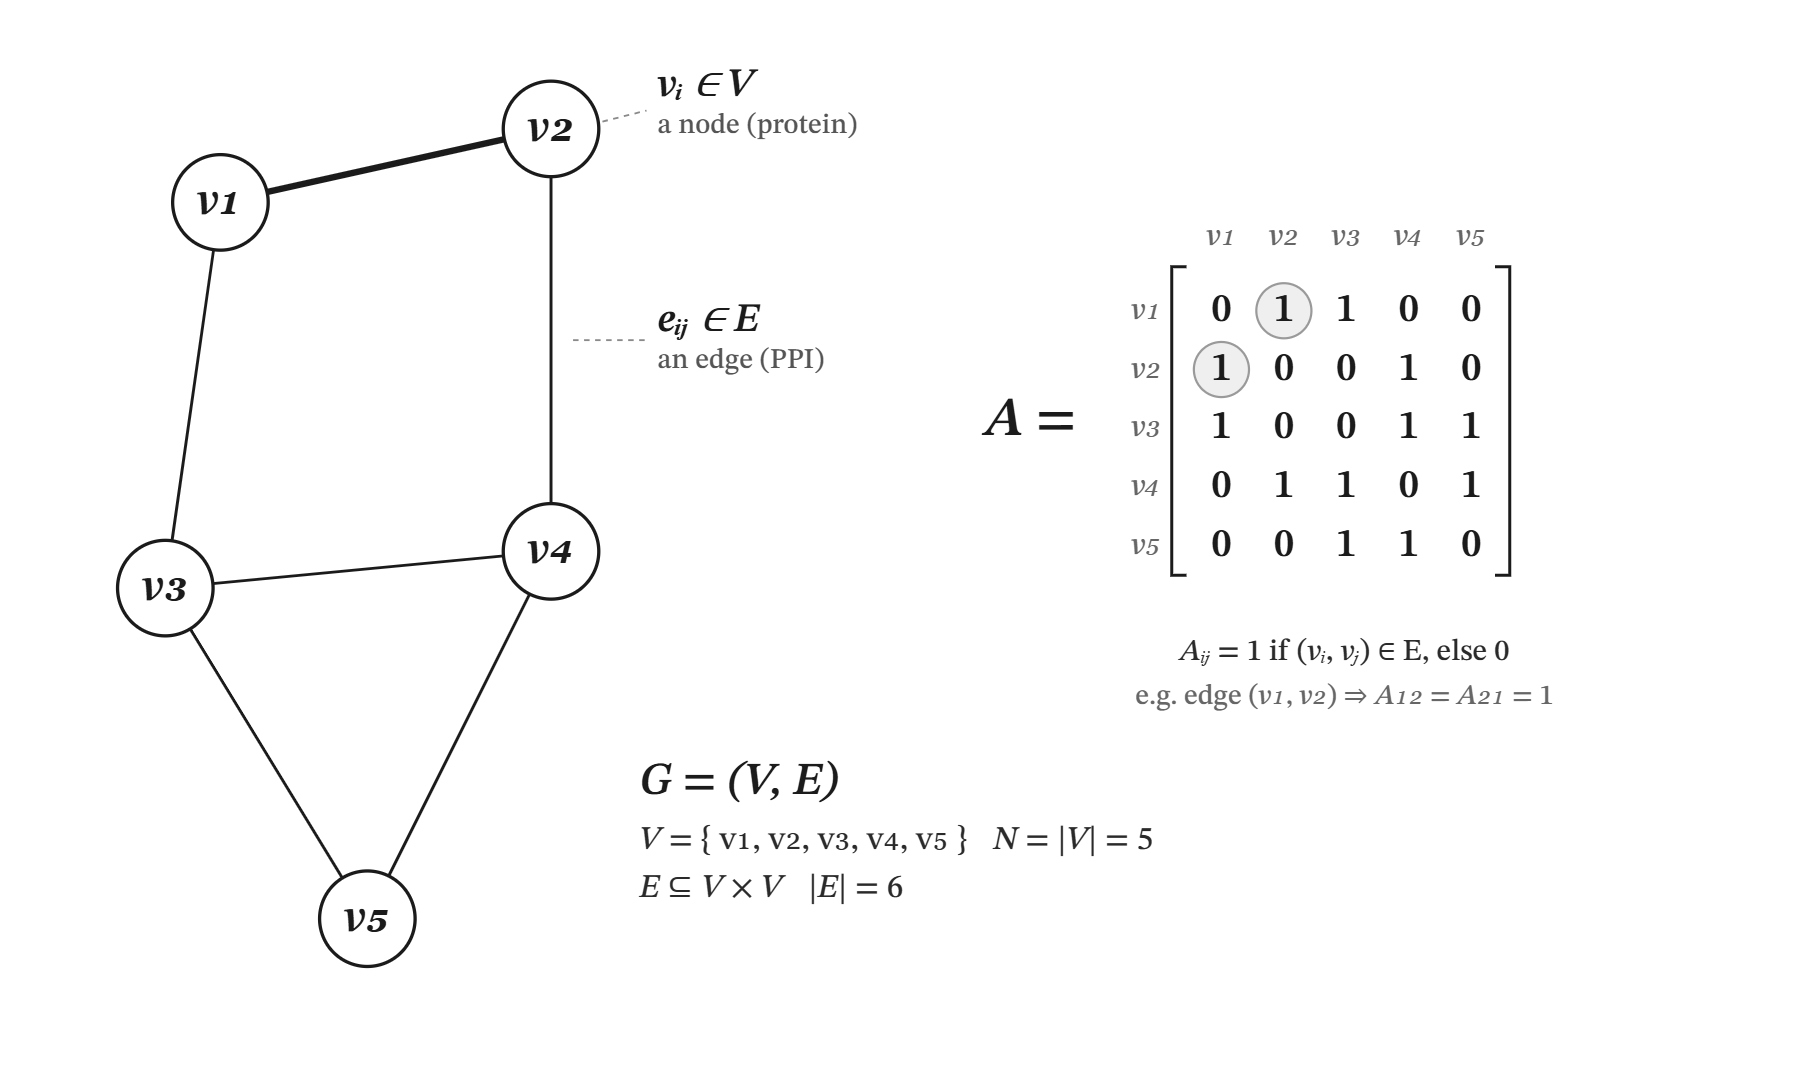
\includegraphics[width=\linewidth]{fig_2_3}\\
    {\scriptsize Fig.~2.3: graph notation and adjacency.}
  \end{columns}
  \src{§2.2.1; §2.2.3}
\end{frame}

\begin{frame}{Building blocks}
  \begin{columns}[T]
    \column{0.3\textwidth}
    \textbf{MLP}\\ the vector prediction head
    \vspace{1em}

    \textbf{CNN}\\ backbone of the image route (ResNet-50, ConvNeXt-Tiny)
    \vspace{1em}

    \textbf{Autoencoder}\\ the compression inside deepNF, one of the baselines
    \column{0.68\textwidth}
    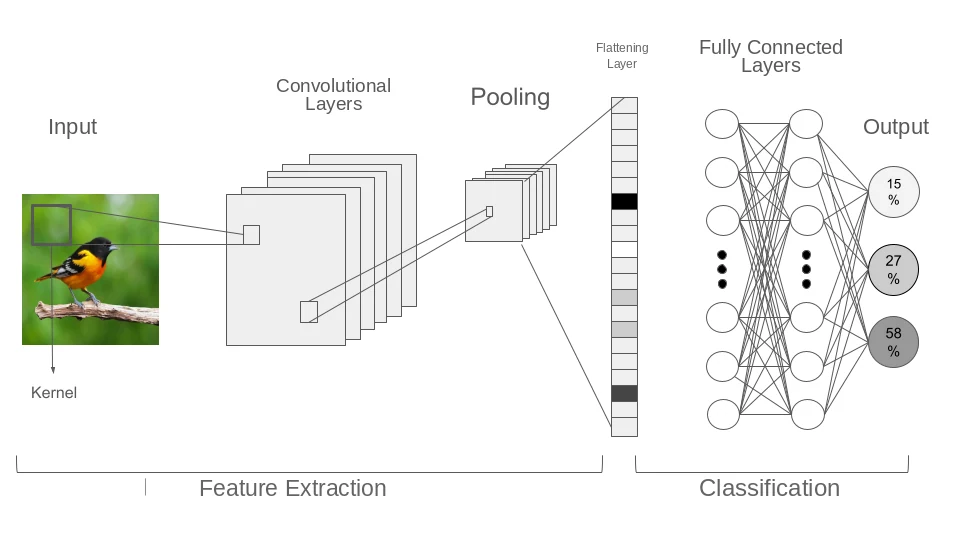
\includegraphics[height=0.32\textheight]{fig_2_6}\\[0.3em]
    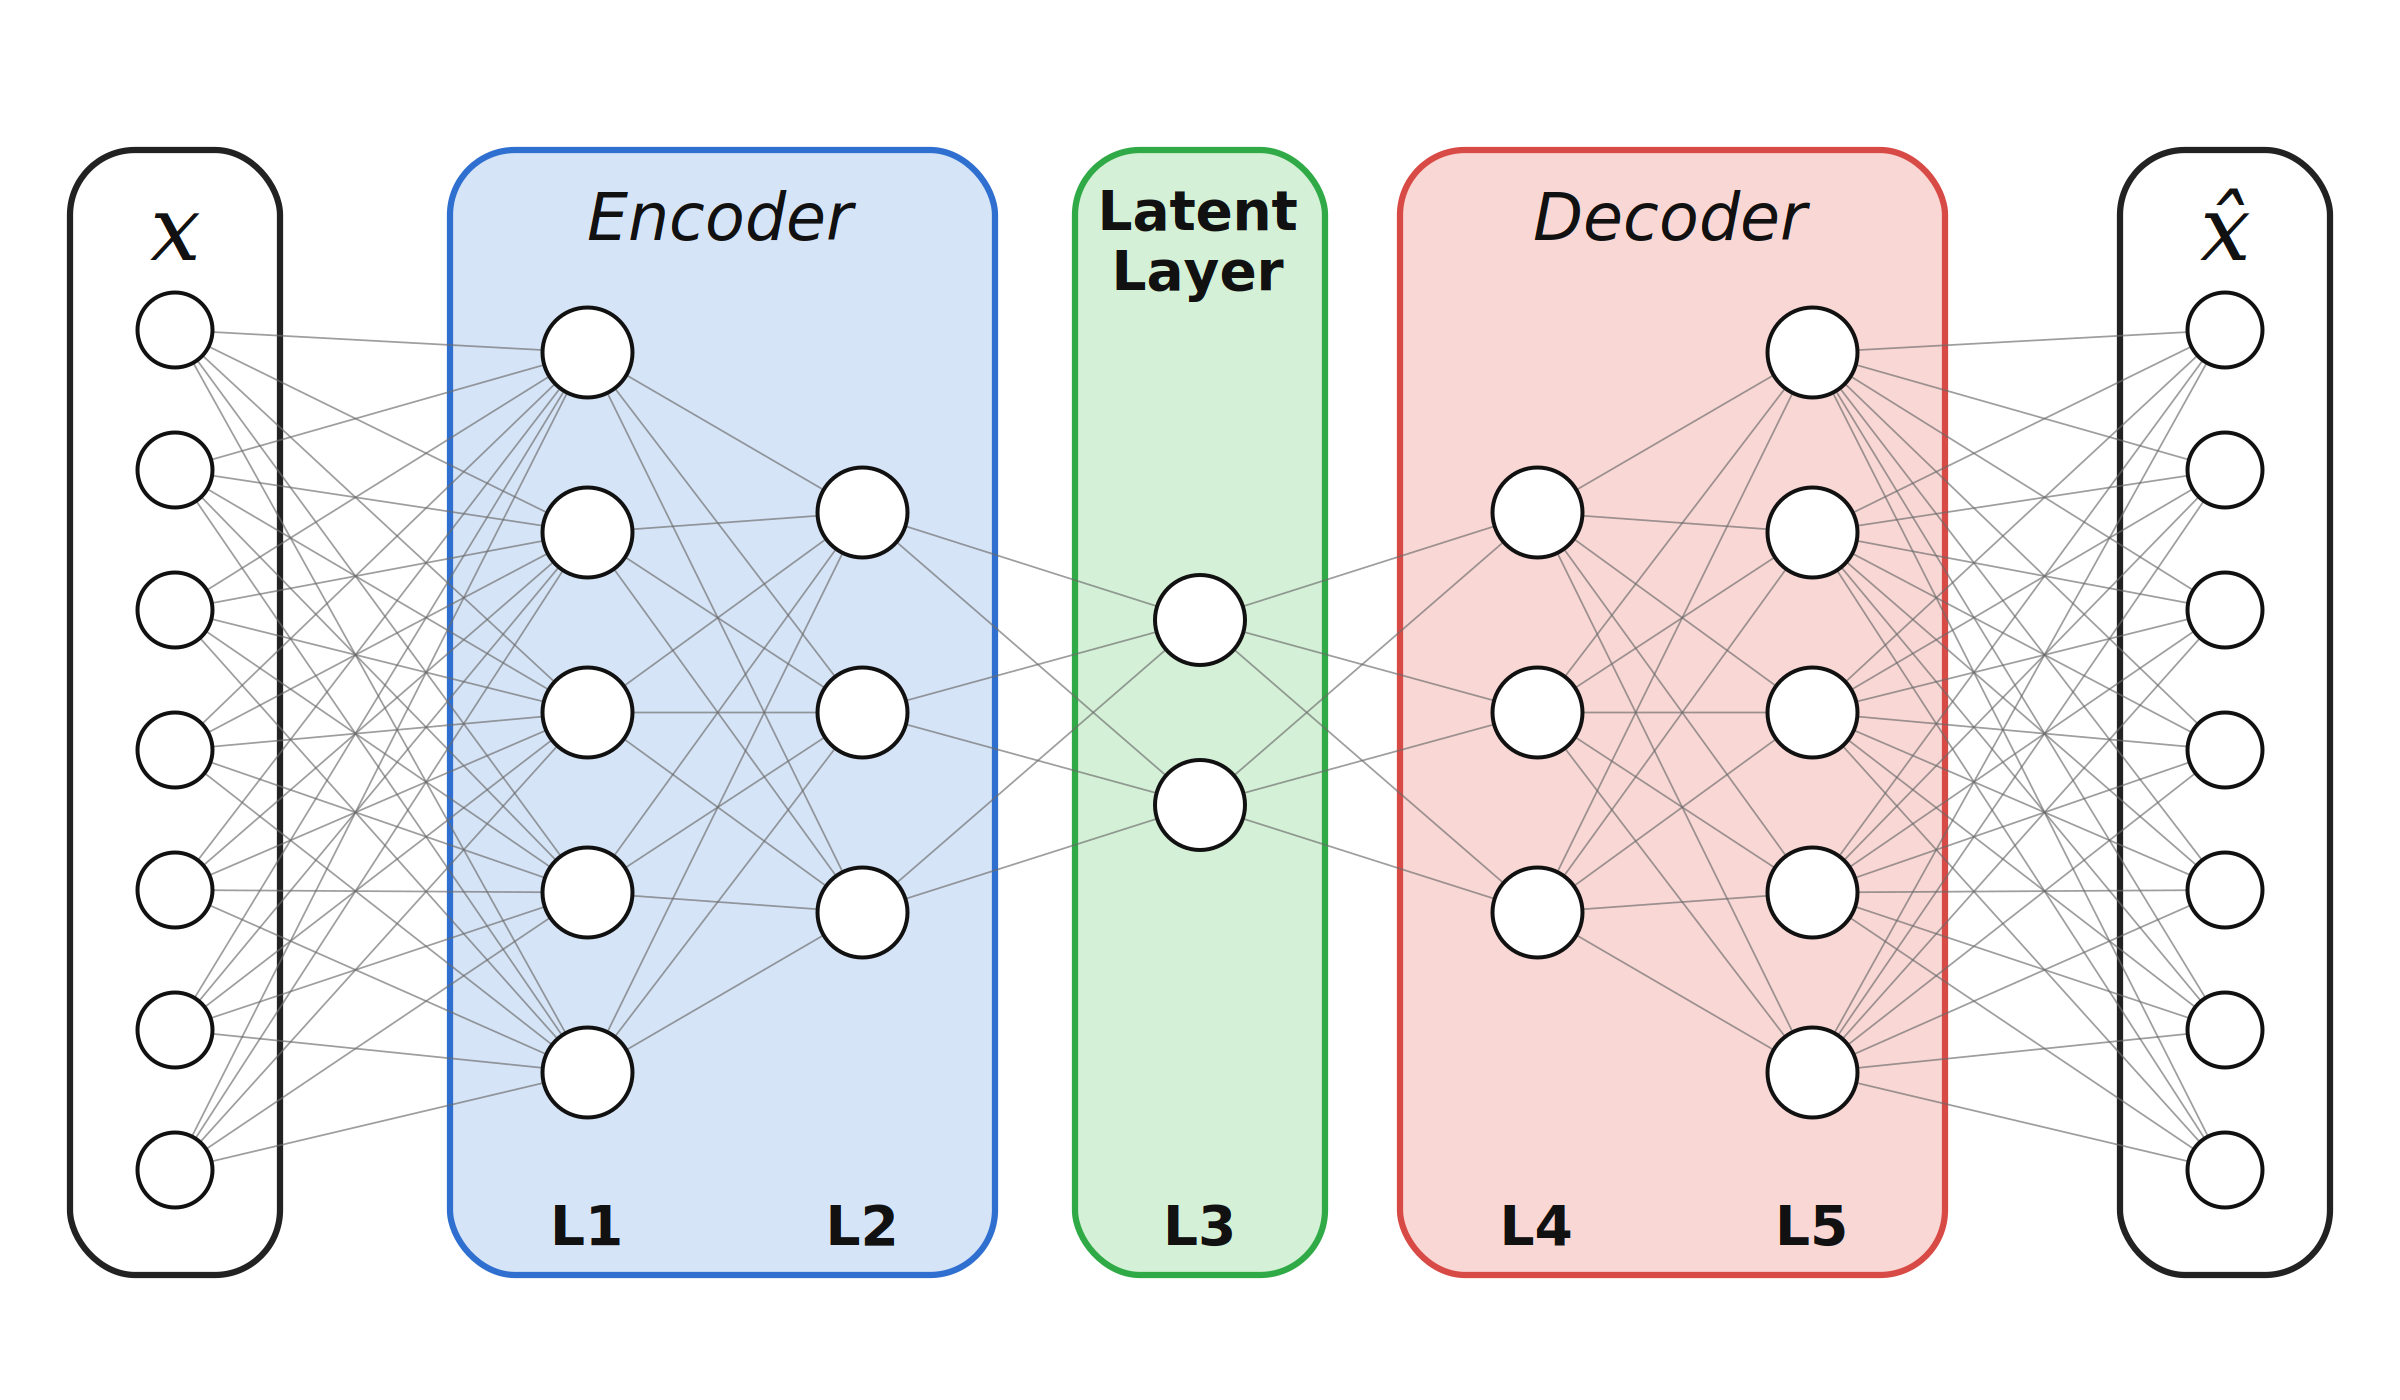
\includegraphics[height=0.32\textheight]{fig_2_7}\\
    {\scriptsize Figs.~2.6 and 2.7: CNN pipeline and autoencoder.}
  \end{columns}
  \src{§2.2.3, §2.2.4}
\end{frame}

\begin{frame}{Protein language models}
  \begin{itemize}
    \item Self-supervised pretraining on hundreds of millions of sequences
    \item Transformer encoder: every residue attends to every other
    \item ProtT5-XL-U50: T5 encoder, BFD then UniRef50, 15\% residue masking
    \item Used here as a \alert{frozen} feature extractor
  \end{itemize}
  \src{§2.2.4, §2.2.5; §3.1.1; §5.4.1}
\end{frame}

\begin{frame}{From neighbour voting to graph transformers}
  \begin{center}
  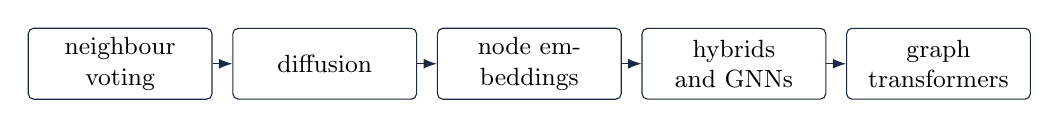
\begin{tikzpicture}[node distance=0.25cm, box/.style={draw=ink, rounded corners=2pt, align=center, font=\small, minimum height=0.9cm, text width=2.1cm}]
    \node[box] (a) {neighbour voting};
    \node[box, right=of a] (b) {diffusion};
    \node[box, right=of b] (c) {node embeddings};
    \node[box, right=of c] (d) {hybrids and GNNs};
    \node[box, right=of d] (e) {graph transformers};
    \foreach \x/\y in {a/b,b/c,c/d,d/e} \draw[-{Latex}, ink] (\x) -- (\y);
  \end{tikzpicture}
  \end{center}
  \begin{itemize}
    \item Each step added parameters, tuning surface and cost
    \item Five methods retrained here, and where their parameters live:
    \begin{itemize}
      \item Mashup, deepNF: none in the diffusion, all in the compression
      \item MELISSA: labels injected into the network construction
      \item DeepGraphGO: between propagation steps
      \item SEGT-GO: in a transformer, after a non-parametric multi-hop aggregation
    \end{itemize}
  \end{itemize}
  \src{§3.1.2, §3.1.3, §3.2, §3.3}
\end{frame}

\begin{frame}{The open question}
  \begin{block}{}
    \centering\large Is a learned graph component still needed\\once the propagated object is informative?
  \end{block}
  \vspace{0.5em}
  \begin{itemize}[<+(1)->]
    \item Proposal: propagate ProtT5 embeddings with a fixed, finite-step operator, then use an ordinary head
    \item A sequence representation exists for every protein, so the network adds instead of supplies
    \item No prior visual route starts from a propagated language-model embedding
  \end{itemize}
  \src{§3.3}
\end{frame}

% ============================================================================ Data
\section{Data and evaluation}

\begin{frame}{Data: a CAFA5-derived corpus}
  \begin{center}\small\TabCorpus\end{center}
  \begin{itemize}
    \item 80\,/\,10\,/\,10 split, disjoint at protein level, no temporal or homology constraint
    \item Labels per protein (mean): 25.91 BP, 12.48 CC, 7.55 MF
    \item Label matrix density: 5.18\%, 2.51\%, 1.51\%
  \end{itemize}
  \src{Tables 4.1 and 4.2; §4.1.1, §4.1.2}
\end{frame}

\begin{frame}{STRING v11.5: one aggregated network}
  \begin{itemize}
    \item 2,422,234 records, 791,011 distinct pairs, 86,423 proteins
    \item Combined score in $[0.400, 0.999]$; confidence, not binding strength
    \item Each pair repeated 3.06 times on average (up to 170), always with the same score
    \item Degree is heavy-tailed: median 5--7, maximum between 763 and 805
  \end{itemize}
  \begin{center}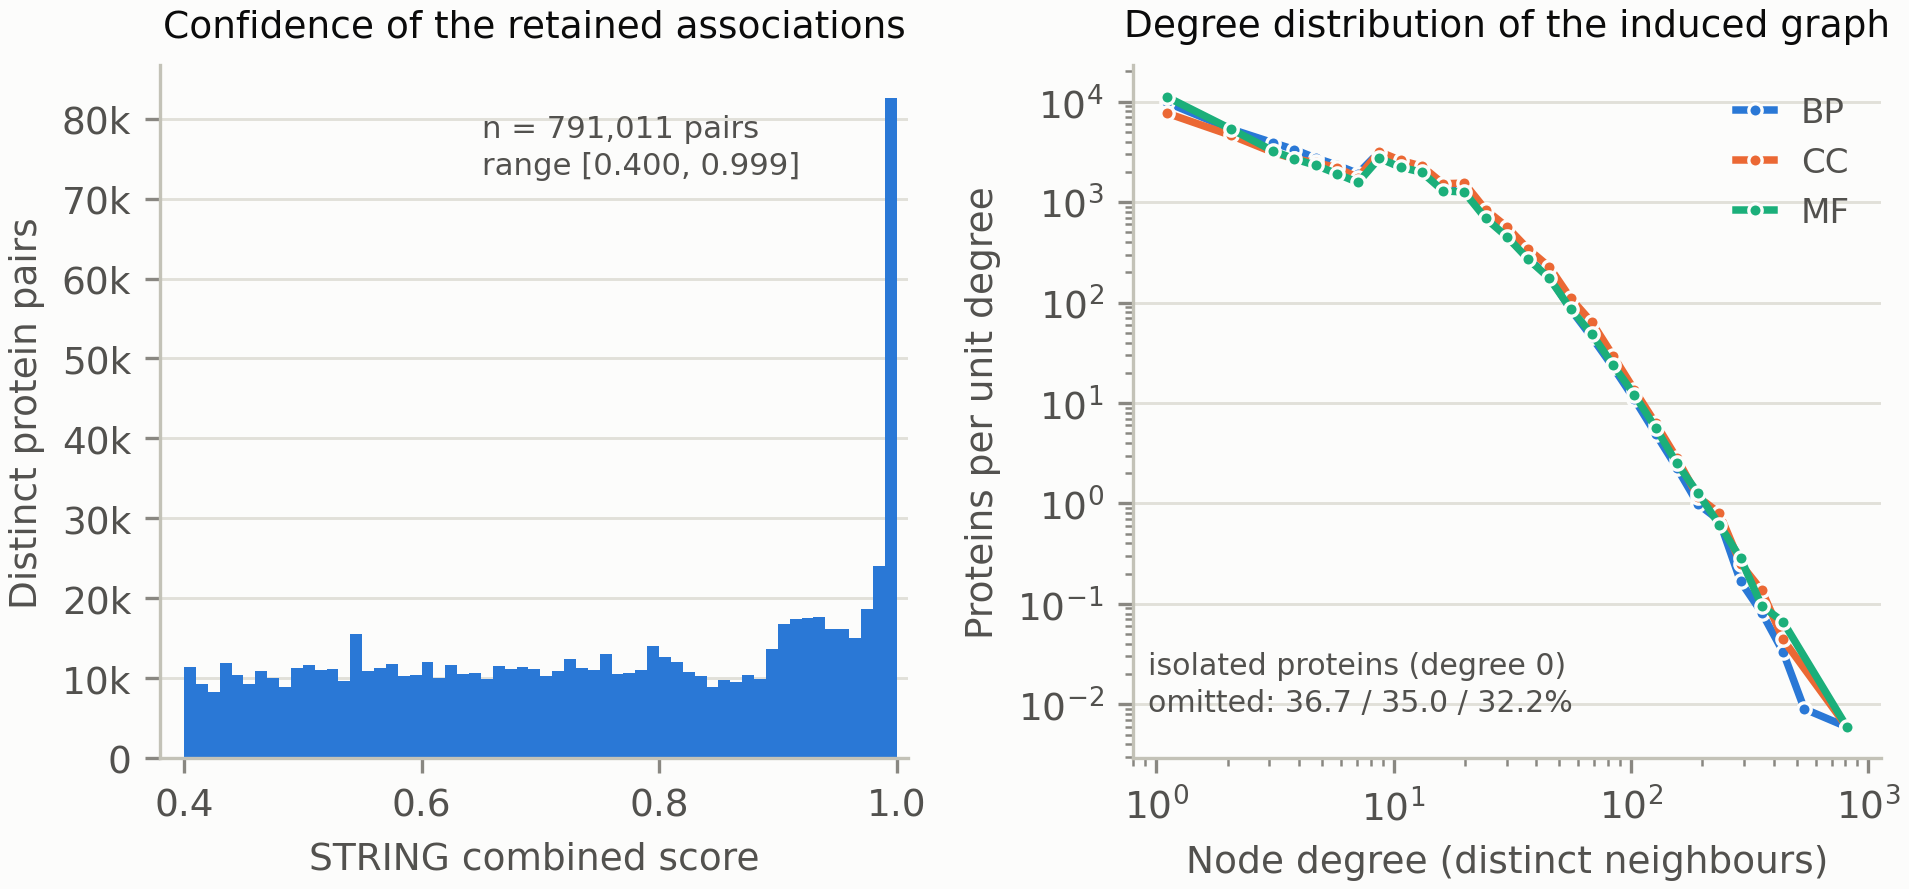
\includegraphics[height=0.5\textheight]{fig_4_1}\end{center}
  \src{§4.1.3; Tables 4.3, 4.4; Fig.~4.1}
\end{frame}

\begin{frame}{One third of the proteins have no edge}
  \begin{itemize}
    \item Isolated: 36.65\% BP, 34.95\% CC, 32.19\% MF; stable across training, validation and test
    \item Thresholds up to 0.40 are inert; at 0.90 more than half the proteins are isolated
  \end{itemize}
  \begin{columns}
    \column{0.49\textwidth}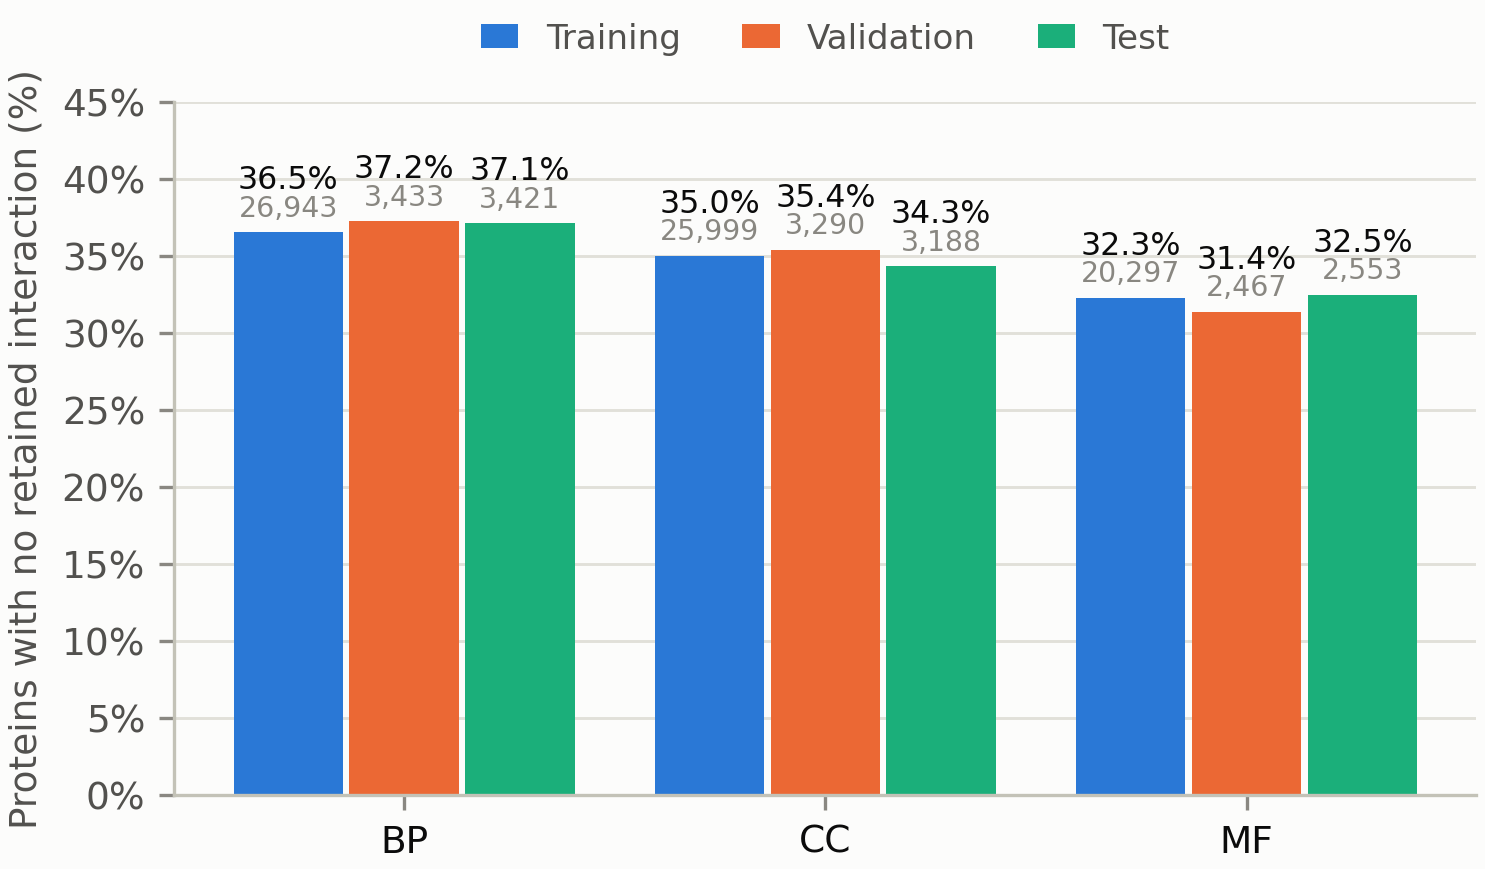
\includegraphics[width=\linewidth]{fig_4_2}
    \column{0.49\textwidth}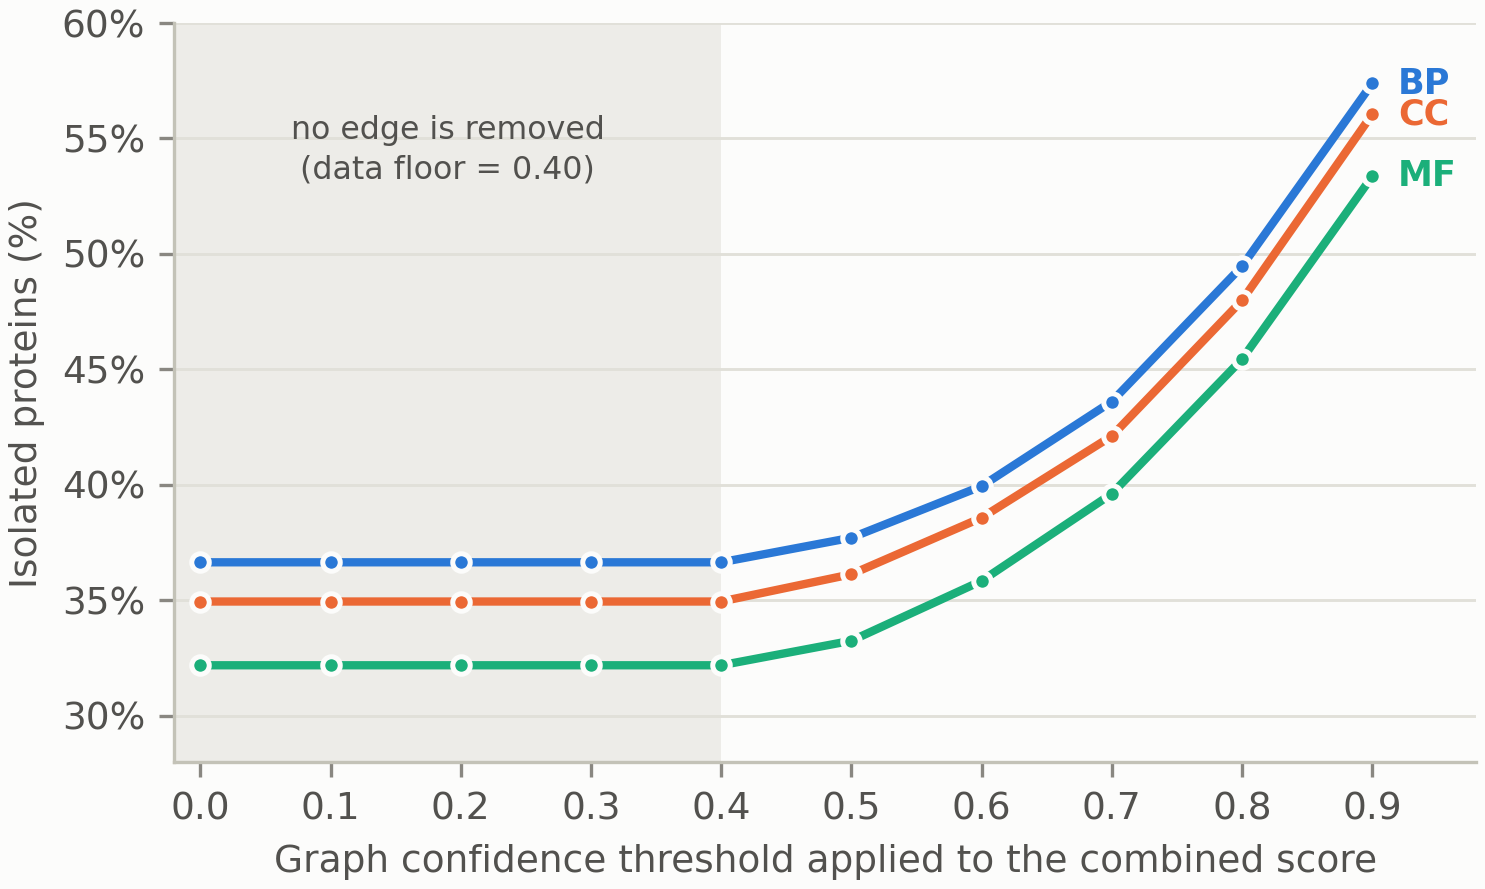
\includegraphics[width=\linewidth]{fig_4_3}
  \end{columns}
  \src{§4.1.3; Table 4.4; Figs.~4.2, 4.3}
\end{frame}

\begin{frame}{Six protein-centric metrics}
  \begin{itemize}
    \item Primary criterion: $\wF$, information-content weighted
  \end{itemize}
  \[
    \wF=\max_{\tau}\frac{2\,\mathrm{wpr}(\tau)\,\mathrm{wrc}(\tau)}{\mathrm{wpr}(\tau)+\mathrm{wrc}(\tau)},
    \qquad \mathrm{IC}(v)=-\log_2 P\big(v\mid \mathrm{pa}(v)\big)
  \]
  \begin{itemize}
    \item Also $F_{\max}$, $F^{*}_{\max}$ (root excluded), $\Smin$ (bits, lower is better), AuPRC, IAuPRC
    \item Predictions made hierarchy-consistent before scoring
    \item 101 thresholds; full evaluation mode (unpredicted proteins count as zero recall)
  \end{itemize}
  \src{§4.2, §4.3; Eqs.~4.8--4.10}
\end{frame}

\begin{frame}{Learning regime and protocol}
  \begin{center}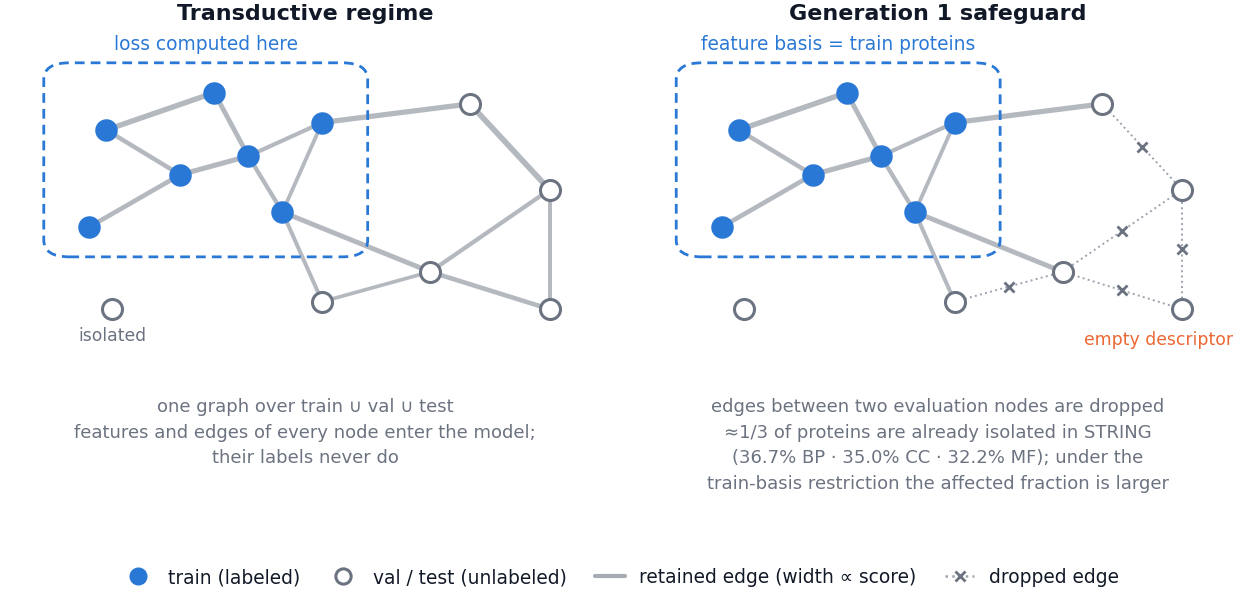
\includegraphics[height=0.42\textheight]{fig_5_2}\end{center}
  \begin{itemize}
    \item One graph over train $\cup$ validation $\cup$ test; labels read only for training proteins
    \item Every design decision on validation; test read once
    \item Single seed: differences below 0.5\,pp are ties (interpretability floor)
  \end{itemize}
  \src{§5.2; §6.1; Fig.~5.2}
\end{frame}

% ============================================================================ Method
\section{Method}

\begin{frame}{Two generations, three decisions}
  \begin{columns}[c]
    \column{0.35\textwidth}
    \begin{itemize}
      \item Representation $\rightarrow$ Propagation $\rightarrow$ Prediction head
      \item Generation 1: network only
      \item $\approx 1/3$ isolated $\rightarrow$ null descriptor
      \item Generation 2 (NEXUS-GO): ProtT5 + network
    \end{itemize}
    \column{0.63\textwidth}
    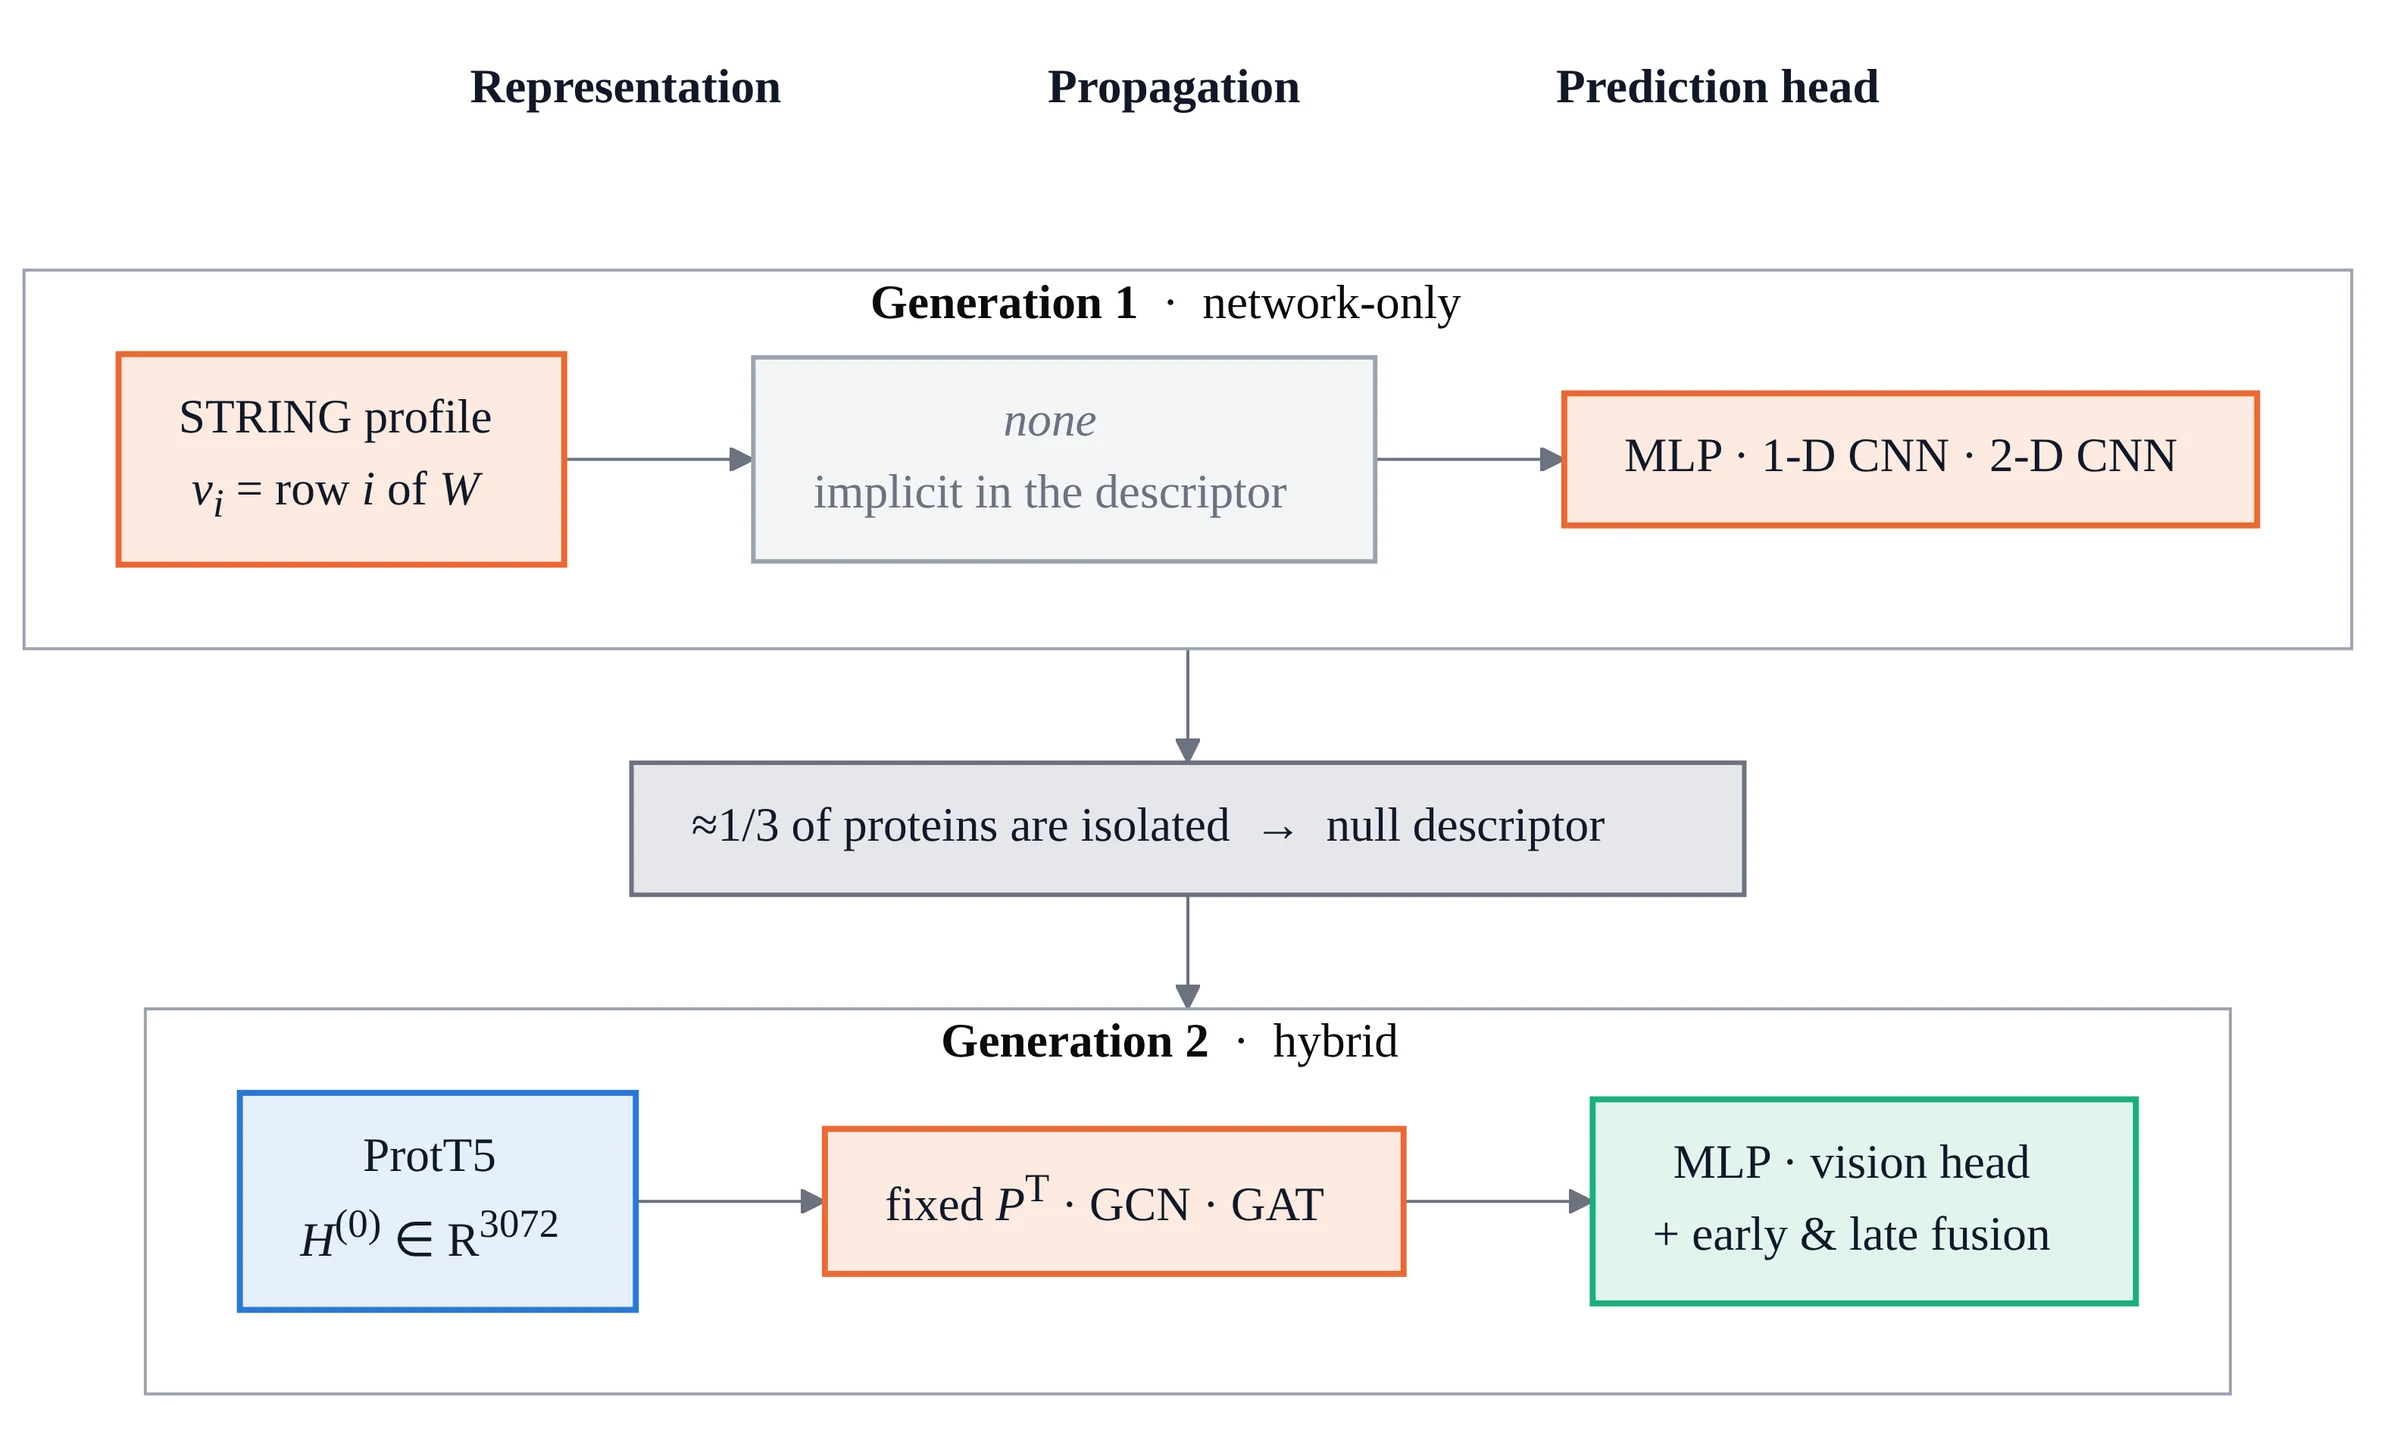
\includegraphics[width=\linewidth]{fig_5_1}
  \end{columns}
  \src{§5.1; Fig.~5.1}
\end{frame}

\begin{frame}{Generation 1: the network alone}
  \begin{columns}[c]
    \column{0.2\textwidth}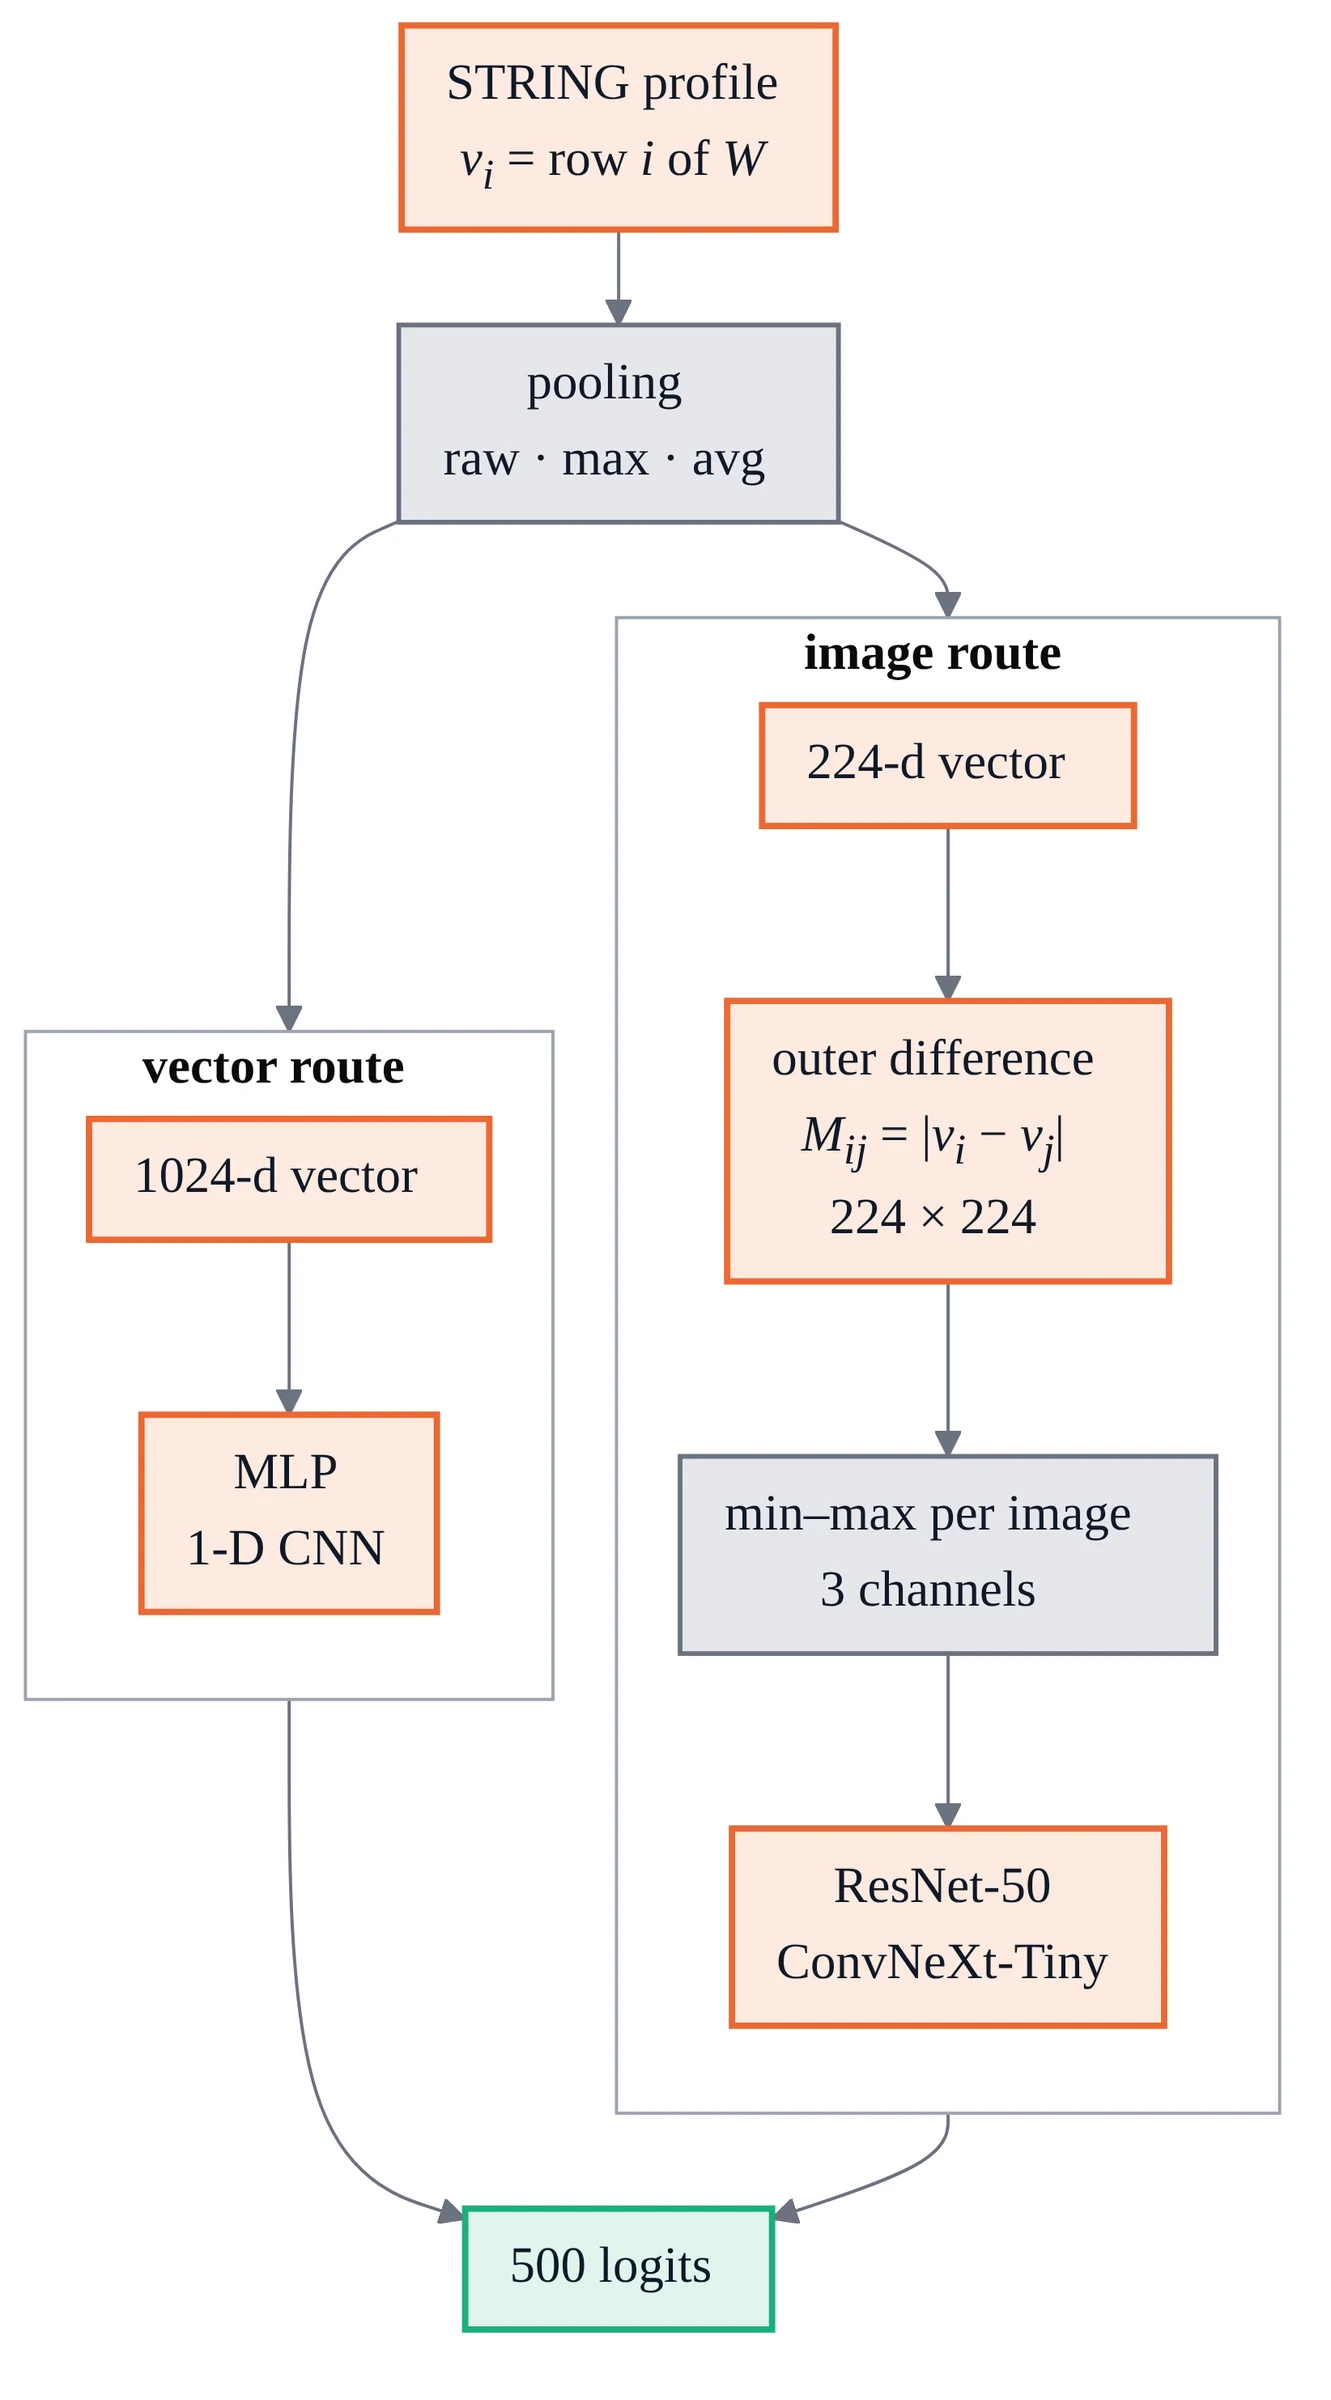
\includegraphics[width=\linewidth,height=0.75\textheight,keepaspectratio]{fig_5_3}
    \column{0.74\textwidth}
    \begin{itemize}
      \item Input: row of the weighted adjacency, against training proteins
      \item Pooling: raw, max, avg
      \item Vector route: MLP or 1-D CNN
      \item Image route: outer-difference matrix $|v_i-v_j|$, $224\times224$, ResNet-50 or ConvNeXt-Tiny
      \item Floor: a naive guilt-by-association baseline
    \end{itemize}
    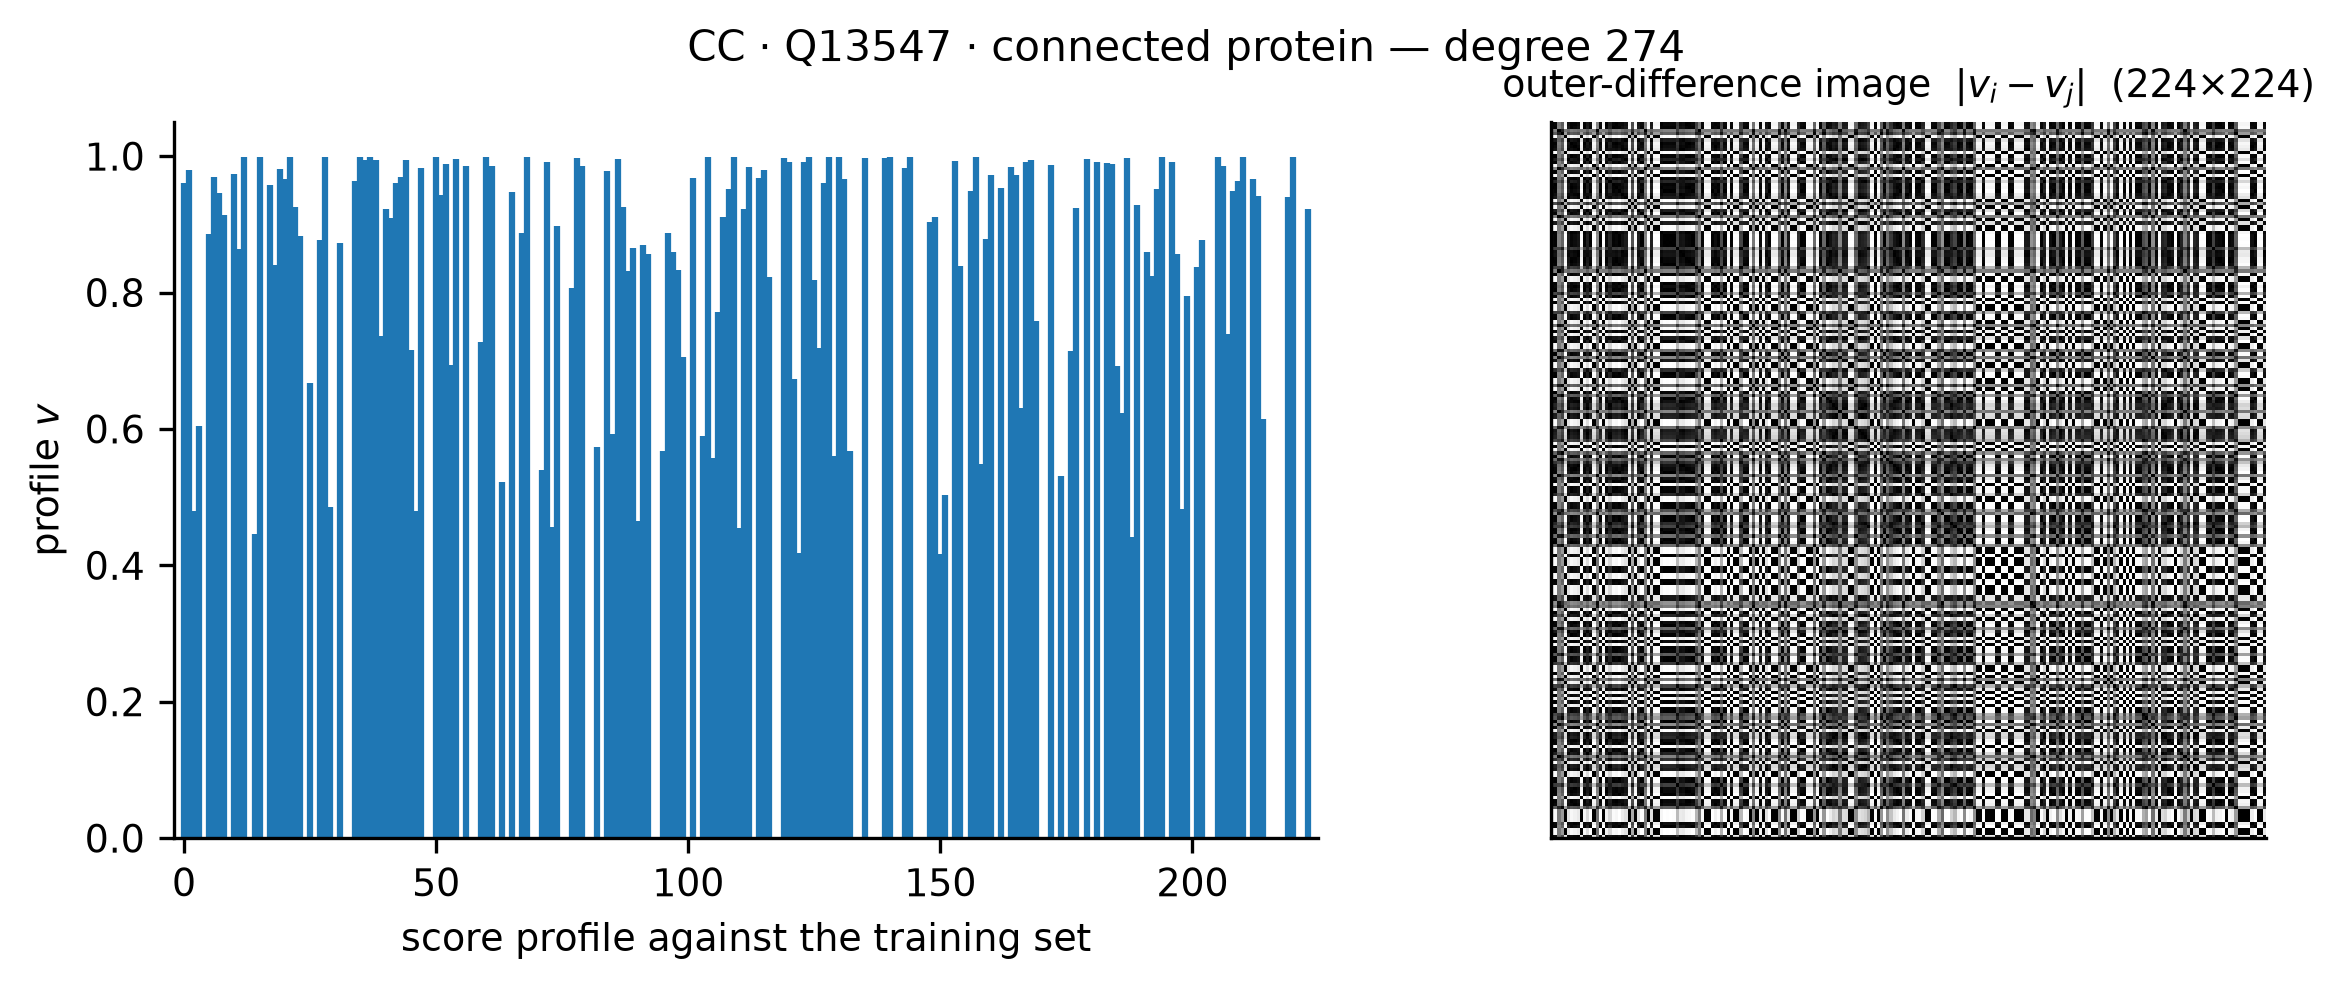
\includegraphics[height=0.3\textheight]{fig_5_4}
  \end{columns}
  \src{§5.3; Figs.~5.3, 5.4}
\end{frame}

\begin{frame}{An isolated protein has no input}
  \begin{center}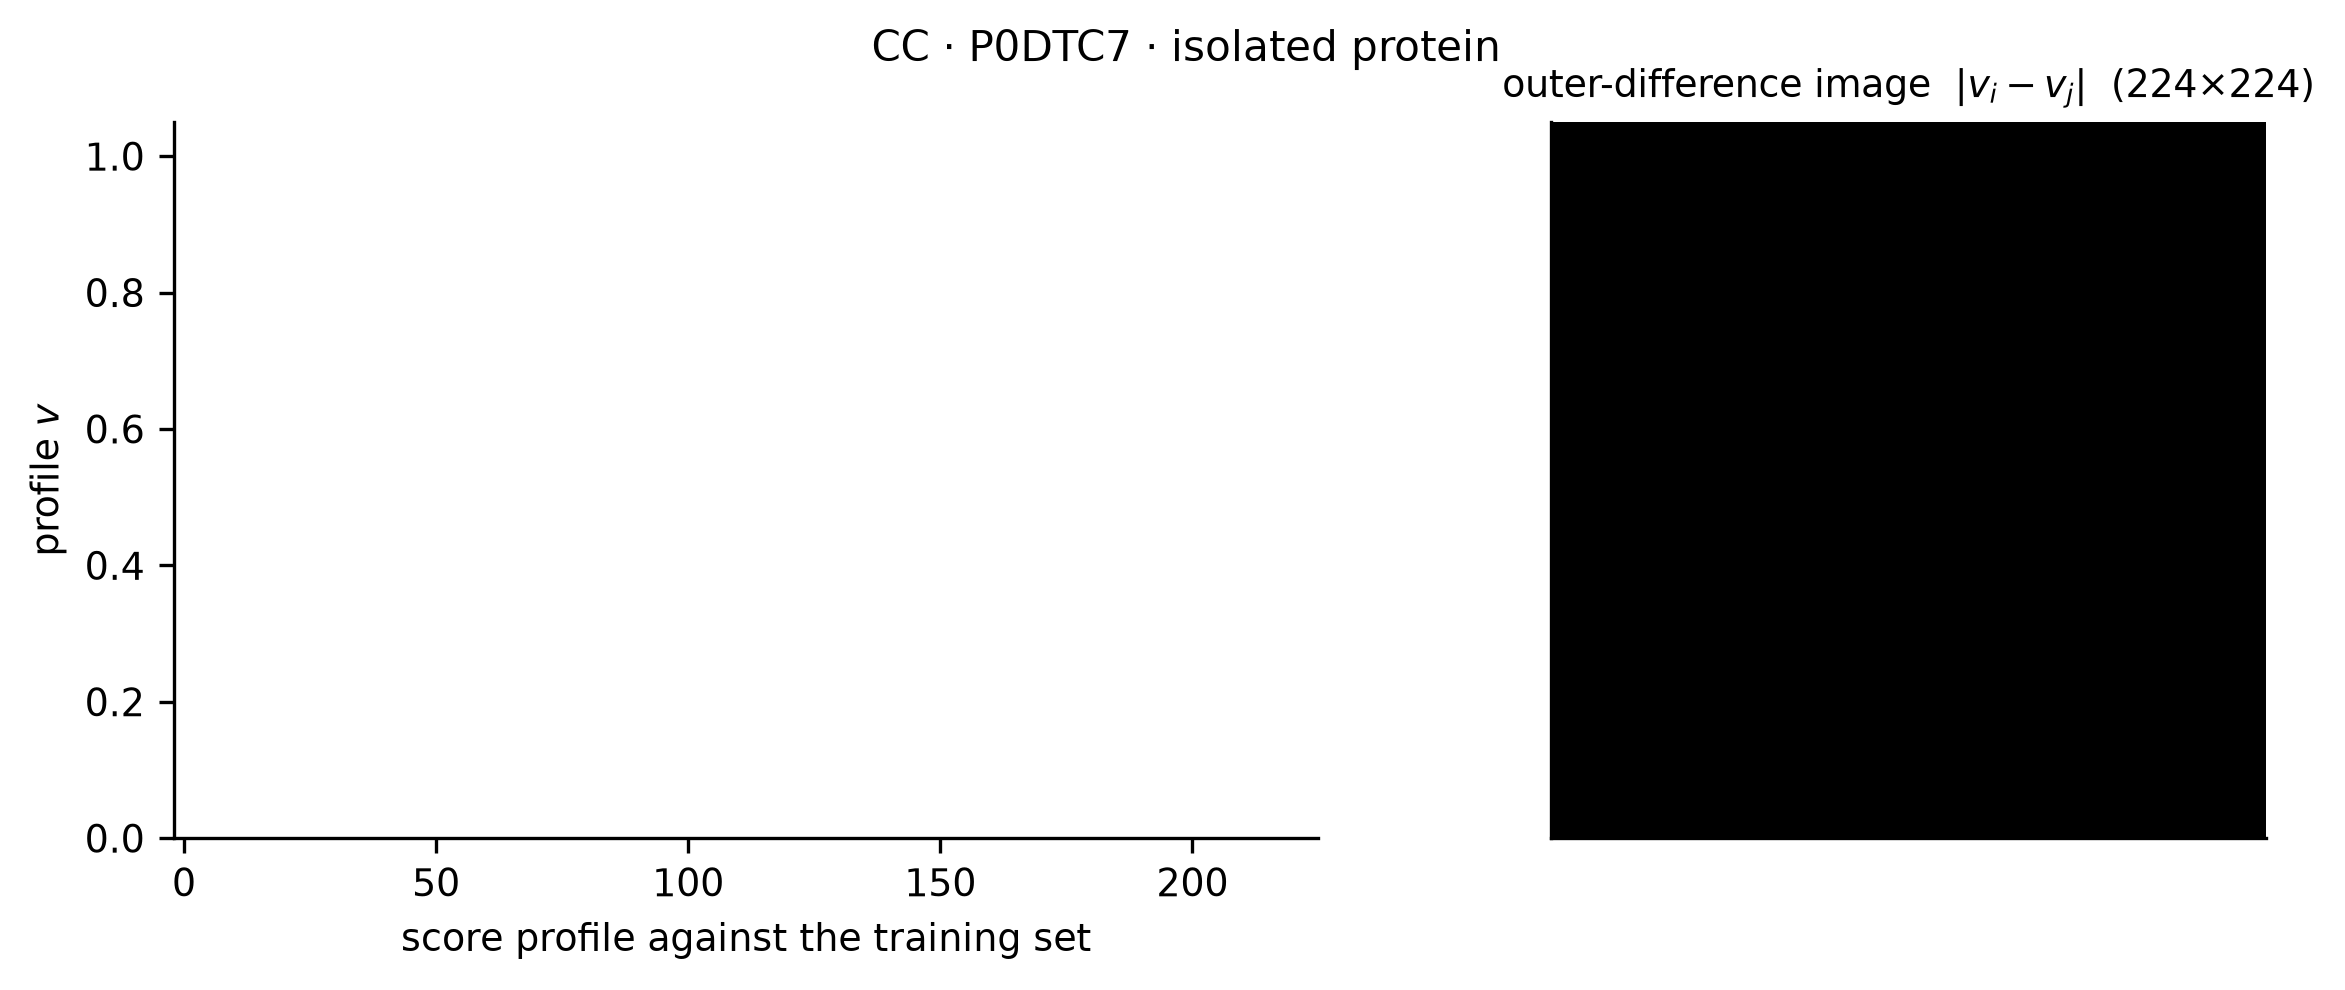
\includegraphics[height=0.45\textheight]{fig_5_5}\end{center}
  \begin{itemize}
    \item Null profile $\rightarrow$ null matrix $\rightarrow$ uniform image: the head can only return the class prior
    \item No architecture can recover what is absent
    \item \alert{Requirement: a representation that exists for every protein}
  \end{itemize}
  \src{§5.3.5; Fig.~5.5}
\end{frame}

\begin{frame}{NEXUS-GO: four routes}
  \begin{center}
  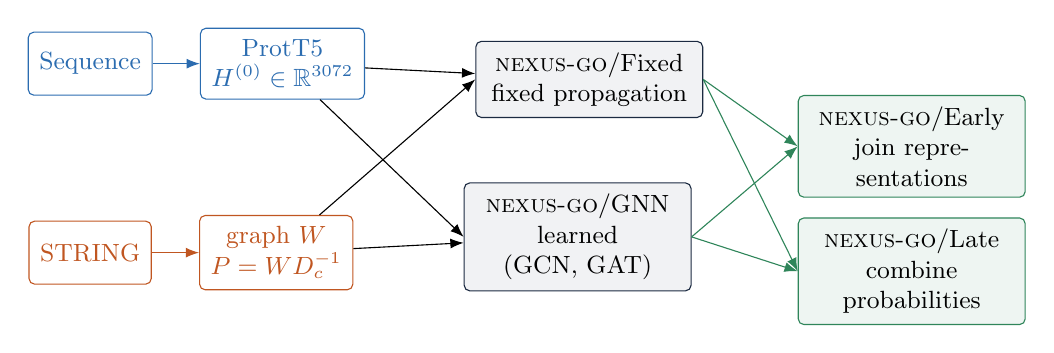
\begin{tikzpicture}[font=\small, >={Latex},
      b/.style={draw, rounded corners=2pt, align=center, minimum height=0.8cm, inner sep=4pt},
      r/.style={b, draw=ink, fill=ink!6, text width=2.6cm}]
    \node[b, draw=seq, text=seq] (seq) at (0,1.2) {Sequence};
    \node[b, draw=seq, text=seq, right=0.6cm of seq] (pt5) {ProtT5\\$H^{(0)}\in\mathbb{R}^{3072}$};
    \node[b, draw=net, text=net] (str) at (0,-1.2) {STRING};
    \node[b, draw=net, text=net, right=0.6cm of str] (w) {graph $W$\\$P=W D_c^{-1}$};
    \draw[->, seq] (seq) -- (pt5); \draw[->, net] (str) -- (w);
    \node[r, right=1.4cm of pt5, yshift=-0.2cm] (fix) {\NX{Fixed}\\fixed propagation};
    \node[r, right=1.4cm of w, yshift=0.2cm] (gnn) {\NX{GNN}\\learned (GCN, GAT)};
    \draw[->] (pt5) -- (fix); \draw[->] (w) -- (fix.west);
    \draw[->] (pt5) -- (gnn.west); \draw[->] (w) -- (gnn);
    \node[r, draw=fus, fill=fus!8, right=1.2cm of fix, yshift=-0.85cm] (early) {\NX{Early}\\join representations};
    \node[r, draw=fus, fill=fus!8, below=0.25cm of early] (late) {\NX{Late}\\combine probabilities};
    \draw[->, fus] (fix.east) -- (early.west); \draw[->, fus] (gnn.east) -- (early.west);
    \draw[->, fus] (fix.east) -- (late.west); \draw[->, fus] (gnn.east) -- (late.west);
  \end{tikzpicture}
  \end{center}
  {\small Generation 1 is reported as a topology-only control and carries no route name.}
  \src{§5.1, §5.4; Fig.~5.6}
\end{frame}

\begin{frame}{ProtT5-XL-U50, three layers, frozen}
  \begin{center}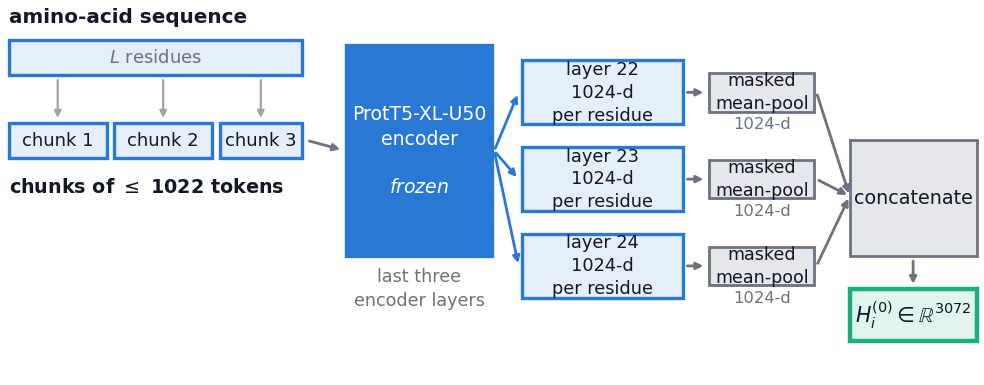
\includegraphics[width=0.7\linewidth]{fig_5_7}\end{center}
  \begin{itemize}
    \item Chunks of at most 1,022 residues; masked mean-pool, then mean over chunks
    \item Layers 24, 23, 22, concatenated: $3\times1024=3072$ dimensions
    \item Exists for every protein, isolated or not
  \end{itemize}
  \src{§5.4.1; Appendix A.4; Fig.~5.7}
\end{frame}

\begin{frame}{From records to an operator}
  \begin{itemize}
    \item Symmetric weights, no self-loops, sparse COO ($\le$ 1.13\,M stored entries; dense would be 25--35\,GB)
    \item Deduplication: \textbf{max} keeps the score; \textbf{sum} multiplies it by the record count
    \item Column-stochastic $P = W D_c^{-1}$: weights are relative to each protein's neighbours
  \end{itemize}
  \vspace{0.5em}
  {\small Example: neighbour A (score 0.80, 5 records) and B (0.95, 1 record). With sum, A weighs 4.00 against 0.95 and dominates; with max, B (0.95) ranks above A (0.80). Normalization does not undo the reordering.}
  \src{§5.4.1; Table 6.10}
\end{frame}

\begin{frame}{Fixed propagation: no parameters}
  \[
    H^{(h)} = \alpha\,H^{(h-1)} + (1-\alpha)\,P^{\top}H^{(h-1)},\qquad h=1,\dots,T
  \]
  \begin{itemize}
    \item Closed form: hop $k$ gets weight $\binom{T}{k}\,\alpha^{T-k}(1-\alpha)^{k}$
    \item Computed once, cached, reused every epoch
    \item $T=0$ or $\alpha=1$: the graph is switched off (internal control)
    \item Unlike personalized PageRank, the initial state is never reintroduced
  \end{itemize}
  \src{§5.4.2; Eqs.~5.11, 5.12}
\end{frame}

\begin{frame}{Propagation on four real proteins}
  \begin{columns}[c]
    \column{0.55\textwidth}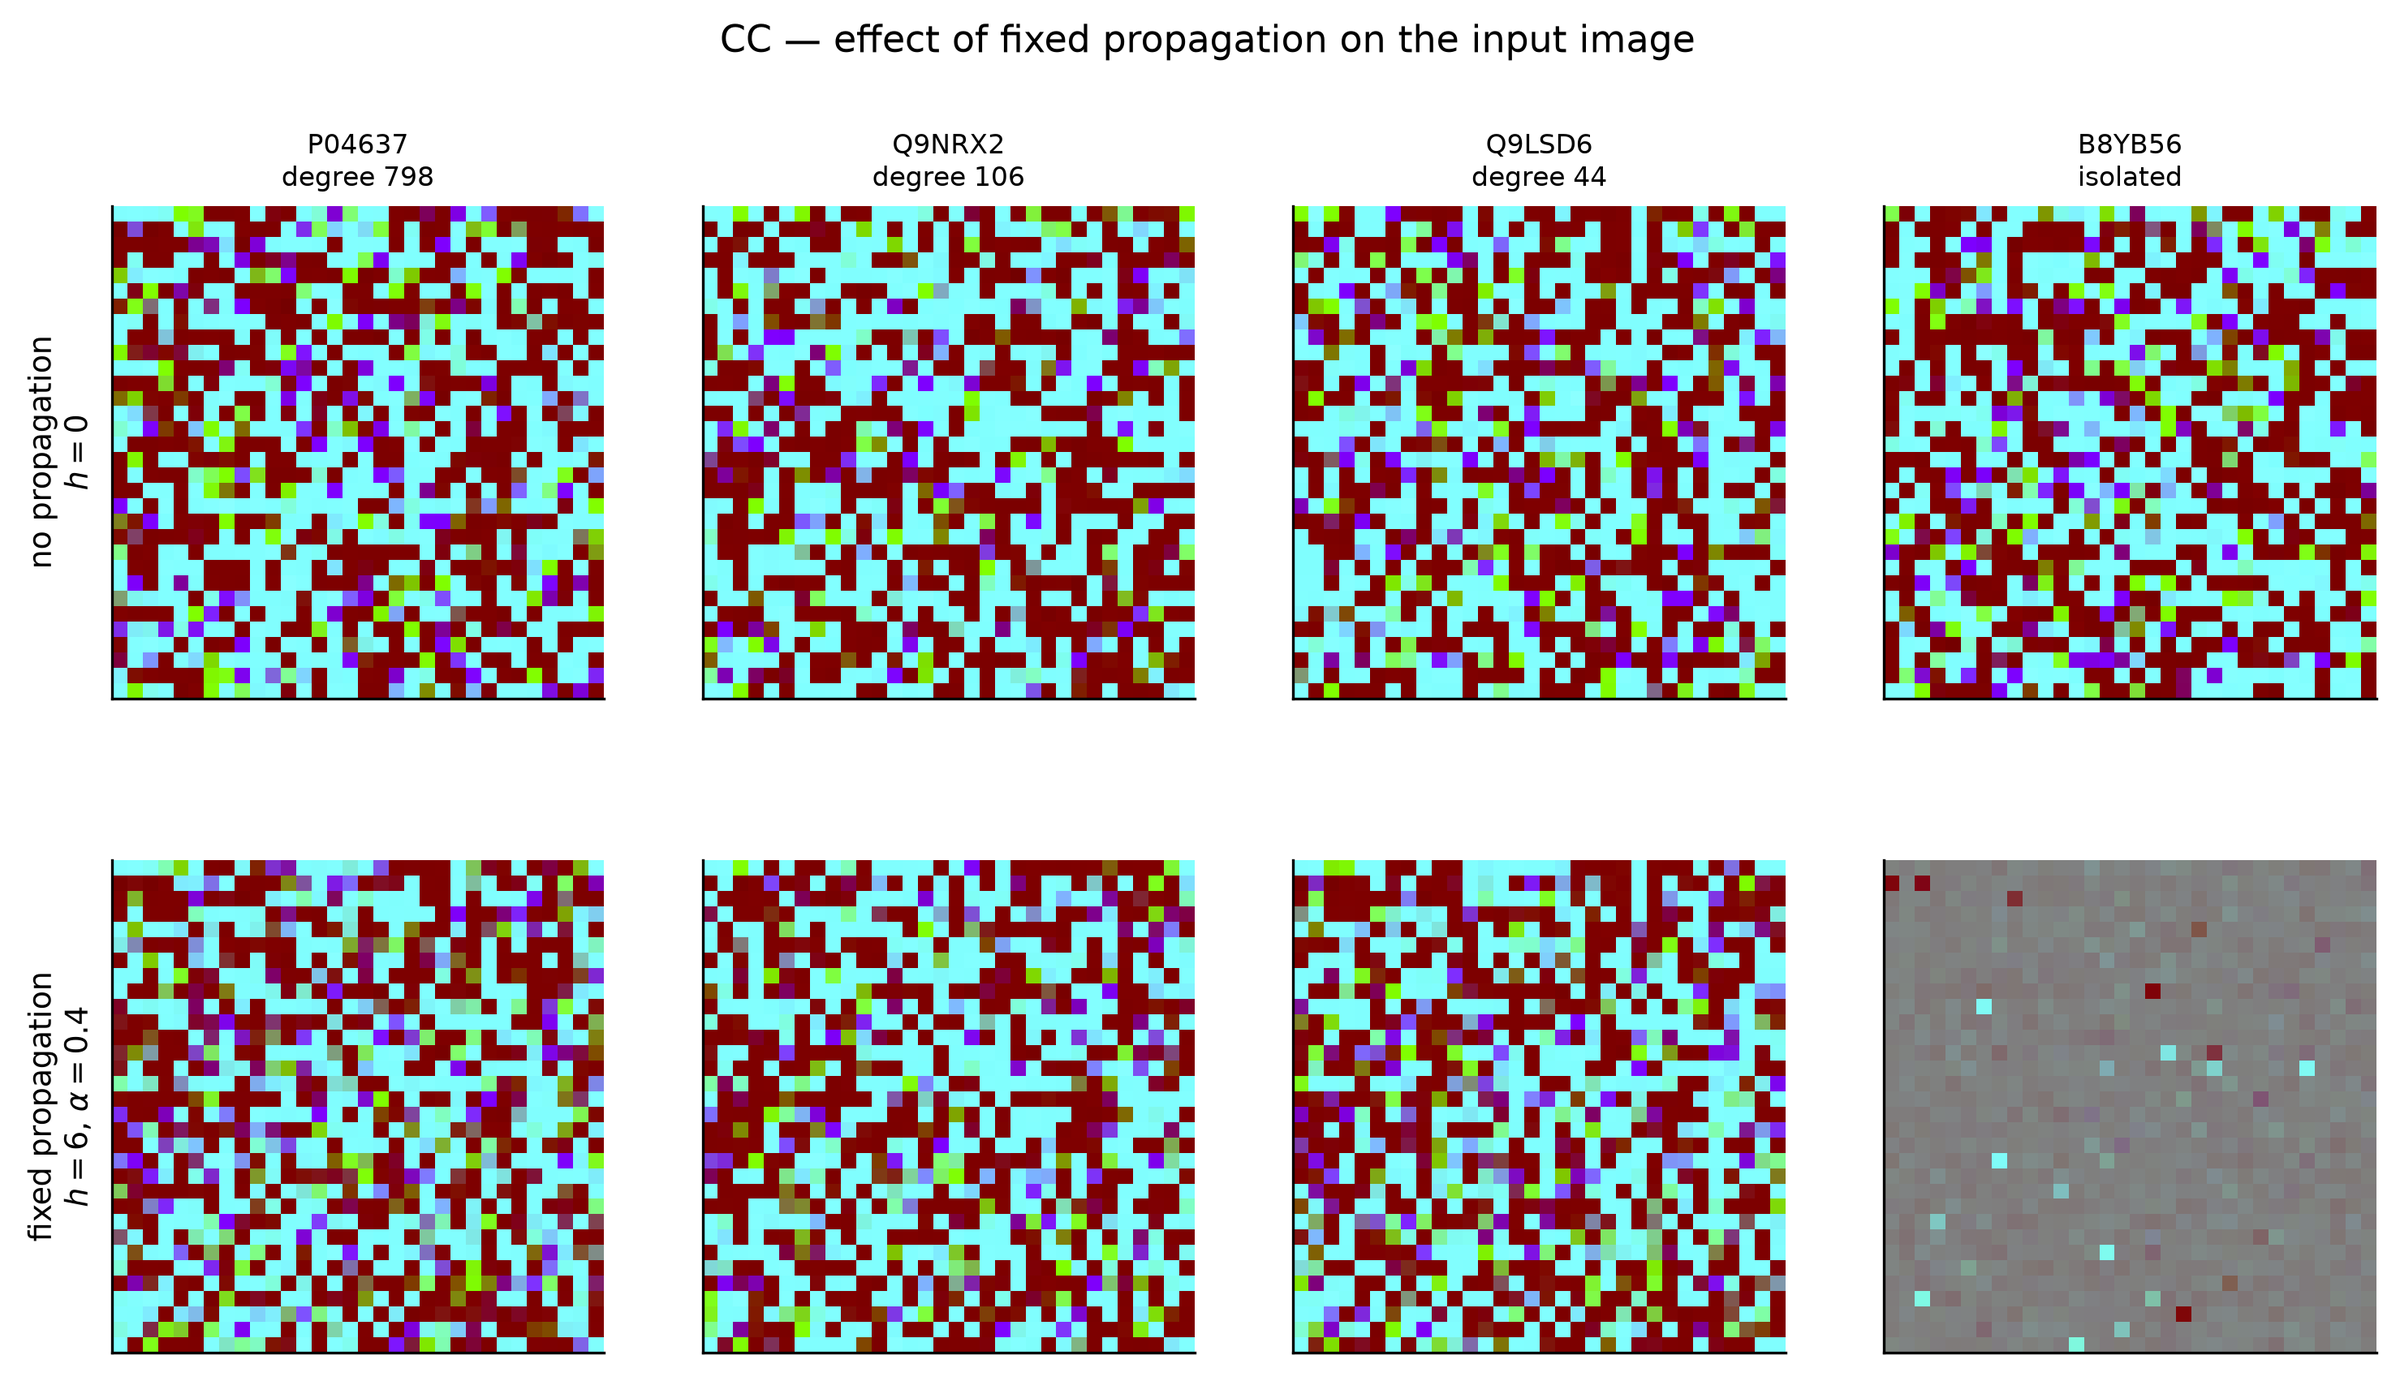
\includegraphics[width=\linewidth]{fig_5_8}
    \column{0.43\textwidth}
    \begin{itemize}
      \item Connected proteins keep their structure and absorb their neighbourhood
      \item An isolated protein becomes $\alpha^{T}H^{(0)}$: same direction, smaller scale
      \item So degree-zero gains cannot come from neighbourhood information
    \end{itemize}
  \end{columns}
  \src{§5.4.2; Fig.~5.8 (CC; $T=0$ top, $T=6$, $\alpha=0.4$ bottom)}
\end{frame}

\begin{frame}{Learned propagation: GCN and GAT}
  \begin{itemize}
    \item GCN: symmetric normalization of $W+I$, then a trained transform
    \item GAT: attention over neighbours, 4 heads, edge score as attribute
    \item 2 layers, width 1024, output $g\in\mathbb{R}^{1024}$ for the head
    \item Full-graph forward on every step: about 289 propagations per epoch
  \end{itemize}
  \vspace{0.6em}
  \centering fixed: \textbf{computed once} \quad·\quad learned: \textbf{recomputed every step}
  \src{§5.4.2; Eqs.~5.14, 5.15; Appendix A.7}
\end{frame}

\begin{frame}{Vector head and vision head}
  \begin{itemize}
    \item Vector: MLP $[1024, 512]$, batch norm, dropout 0.4
    \item Vision: $\sigma(\mathrm{clip}(z))$ split into three $32\times32$ channels, one per ProtT5 layer
    \item Backbones: ResNet-50 and ConvNeXt-Tiny (ImageNet), fully fine-tuned
    \item \alert{Caution}: pixel adjacency has no meaning here
  \end{itemize}
  \begin{center}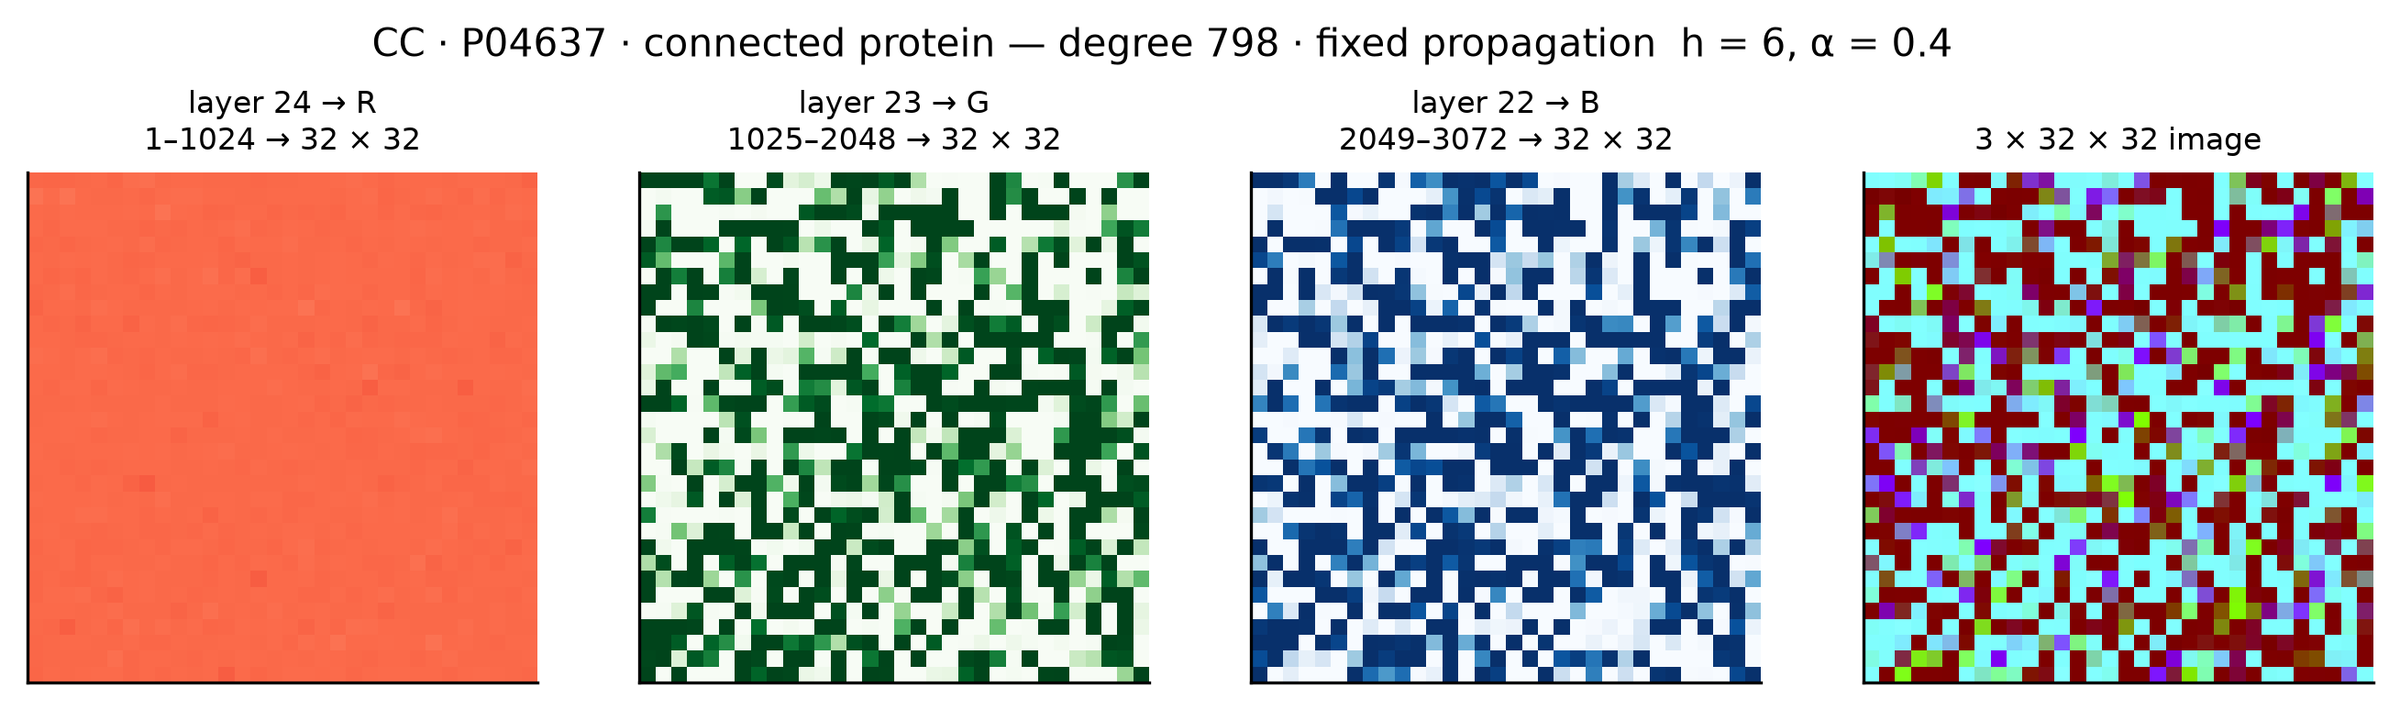
\includegraphics[height=0.33\textheight]{fig_5_9}\end{center}
  \src{§5.4.3; Fig.~5.9}
\end{frame}

\begin{frame}{Training objective: ProteinLoss}
  \[
    \mathcal{L} = \mathcal{L}_{\mathrm{ZLPR}}\cdot\big(1-wF1^{\mathrm{GO}}\big)\cdot\big(1-wF1^{\mathrm{prot}}\big)
  \]
  \begin{itemize}
    \item ZLPR separates positive from negative terms at threshold zero
    \item Two soft, IC-weighted F1 factors: one across terms, one across proteins
    \item Brings training closer to the evaluation criterion
    \item Beats binary cross-entropy by 5.47\,pp on the first-generation mean
  \end{itemize}
  \src{§5.5; Eq.~5.20}
\end{frame}

\begin{frame}{Combining the fixed and learned routes}
  \begin{columns}[c]
    \column{0.42\textwidth}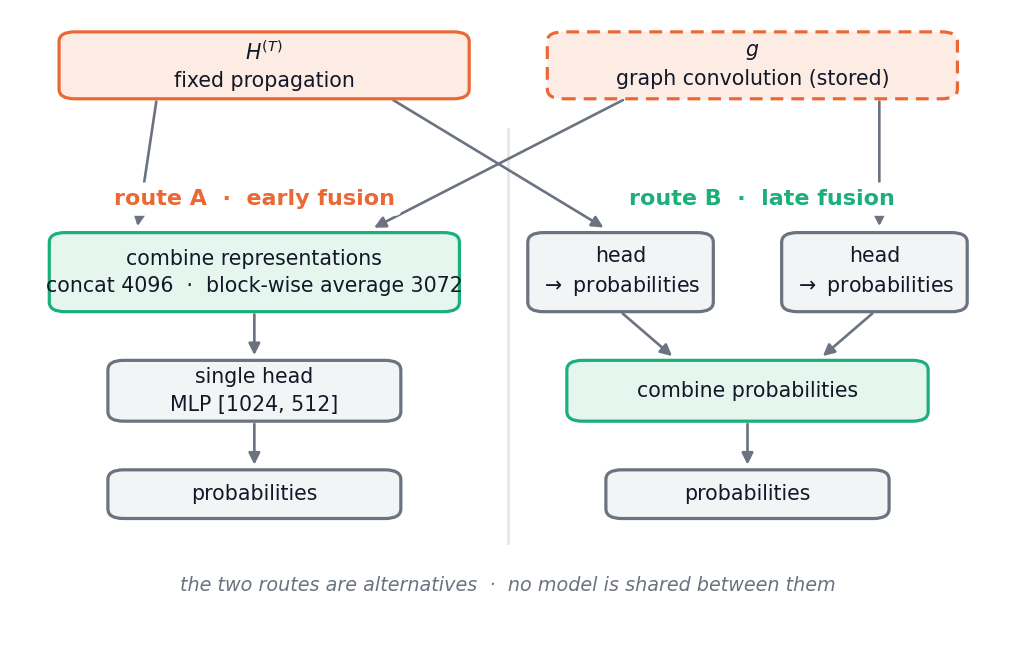
\includegraphics[width=\linewidth]{fig_5_10}
    \column{0.56\textwidth}
    \begin{itemize}
      \item Early: join representations, train one head (concat 4096 or block-wise add 3072)
      \item Late: train each route, combine probabilities
      \item Eleven late rules: linear $\gamma$, max, min, IC sigmoid, degree sigmoid, master equation, five stacking meta-classifiers
      \item Coefficients chosen on validation (71 configurations per ontology)
    \end{itemize}
  \end{columns}
  \src{§5.6; Appendix A.6; Fig.~5.10}
\end{frame}

% ============================================================================ Results
\section{Results}

\begin{frame}{170 runs, one funnel}
  \begin{itemize}
    \item 170 runs, about 136.3 GPU-hours (147 on an RTX A5500)
    \item Each stage picks its winner on validation and hands it on; test read once, at the end
  \end{itemize}
  \vspace{0.4em}
  \begin{center}\scriptsize
  \begin{tabular}{@{}lllll@{}}\toprule
    objective & vector architecture & vision backbone & depth $T$ & retention $\alpha$\\
    ProteinLoss & MLP raw & ConvNeXt-Tiny & per ontology & per ontology\\\midrule
    learned encoder & deduplication & early fusion & late fusion & test\\
    GCN & max & add + GCN + vector & linear $\gamma$ & \NX{Late}\\\bottomrule
  \end{tabular}
  \end{center}
  \src{§5.7; §6.1; Appendix A.7}
\end{frame}

\begin{frame}{Generation 1 settles three choices}
  {\small Mean validation $\wF$}
  \begin{itemize}
    \item Naive term-frequency baseline: 43.56
    \item ProteinLoss beats binary cross-entropy: +5.47\,pp mean (+8.87 in MF)
    \item MLP on the raw profile wins: 44.51; best 1-D CNN 41.16
    \item Vision backbones: 36.99 to 37.62
  \end{itemize}
  \vspace{0.5em}
  Topology alone barely clears a predictor that looks at nothing: +0.95\,pp on the mean.
  \src{Tables 6.1--6.4; §6.2}
\end{frame}

\begin{frame}{One or two hops, high retention (vector head)}
  \begin{columns}
    \column{0.49\textwidth}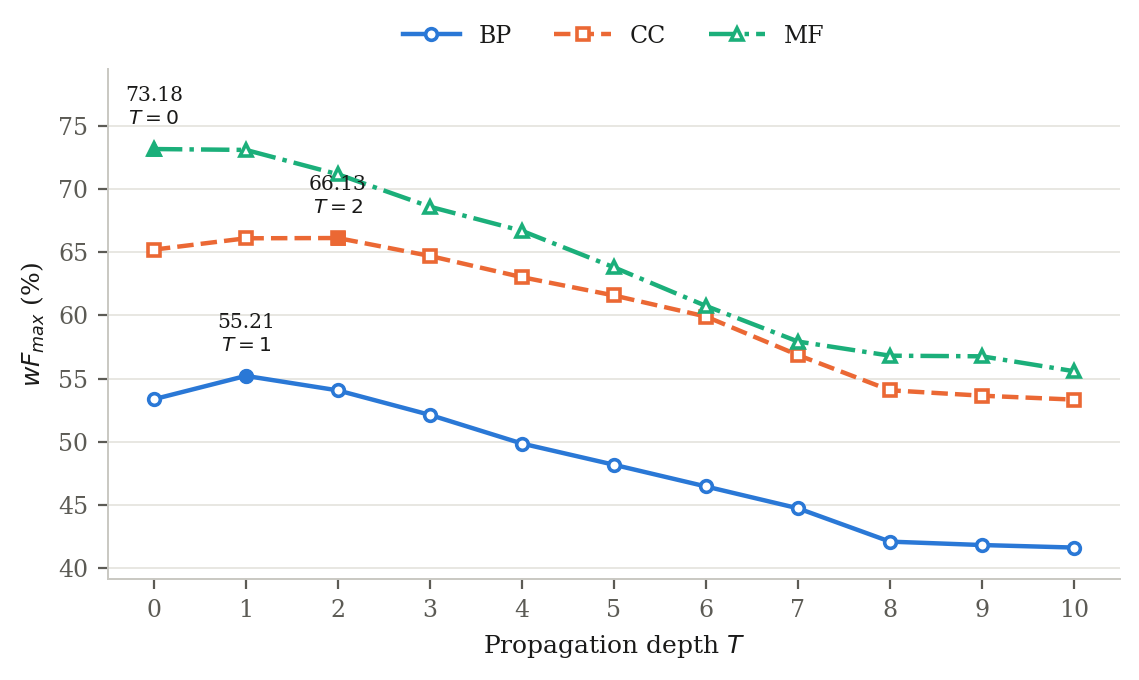
\includegraphics[width=\linewidth]{fig_6_1}
    \column{0.49\textwidth}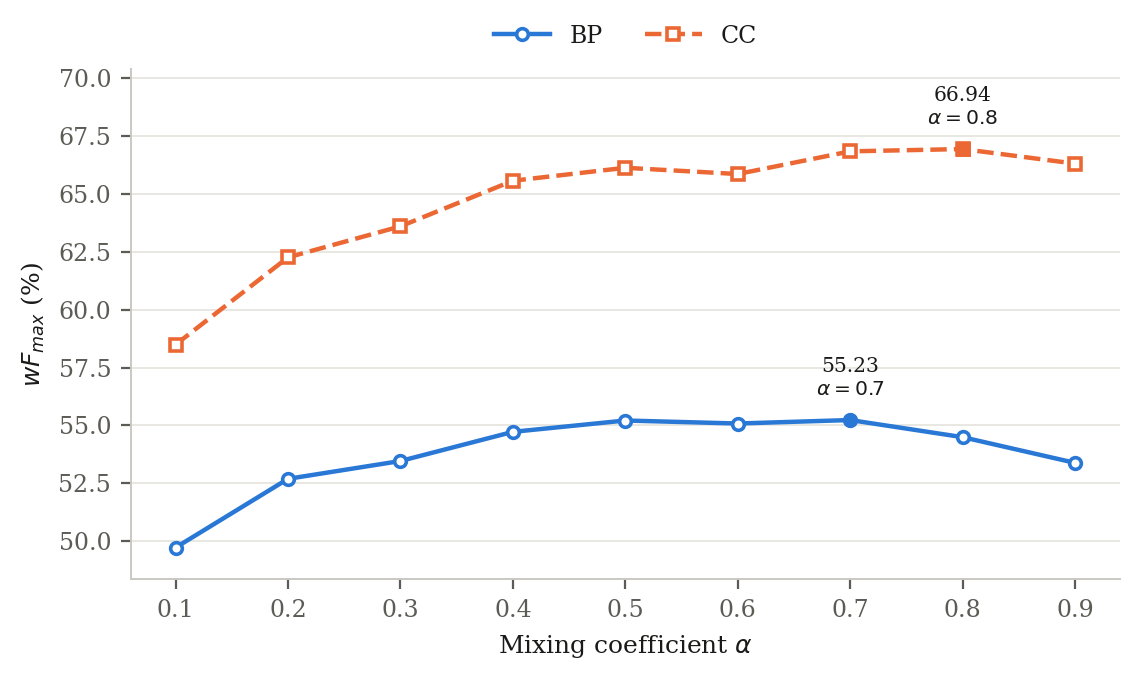
\includegraphics[width=\linewidth]{fig_6_2}
  \end{columns}
  \begin{itemize}
    \item Peak depth: $T=1$ BP, $T=2$ CC, $T=0$ MF; beyond it, 12.80 to 17.60\,pp lost by $T=10$
    \item Best retention: $\alpha=0.7$ BP, $\alpha=0.8$ CC
    \item The graph corrects the protein's own representation; it does not replace it
  \end{itemize}
  \src{Tables 6.5, 6.6; §6.3.1; Figs.~6.1, 6.2}
\end{frame}

\begin{frame}{The vision head wants deep propagation}
  \begin{columns}
    \column{0.49\textwidth}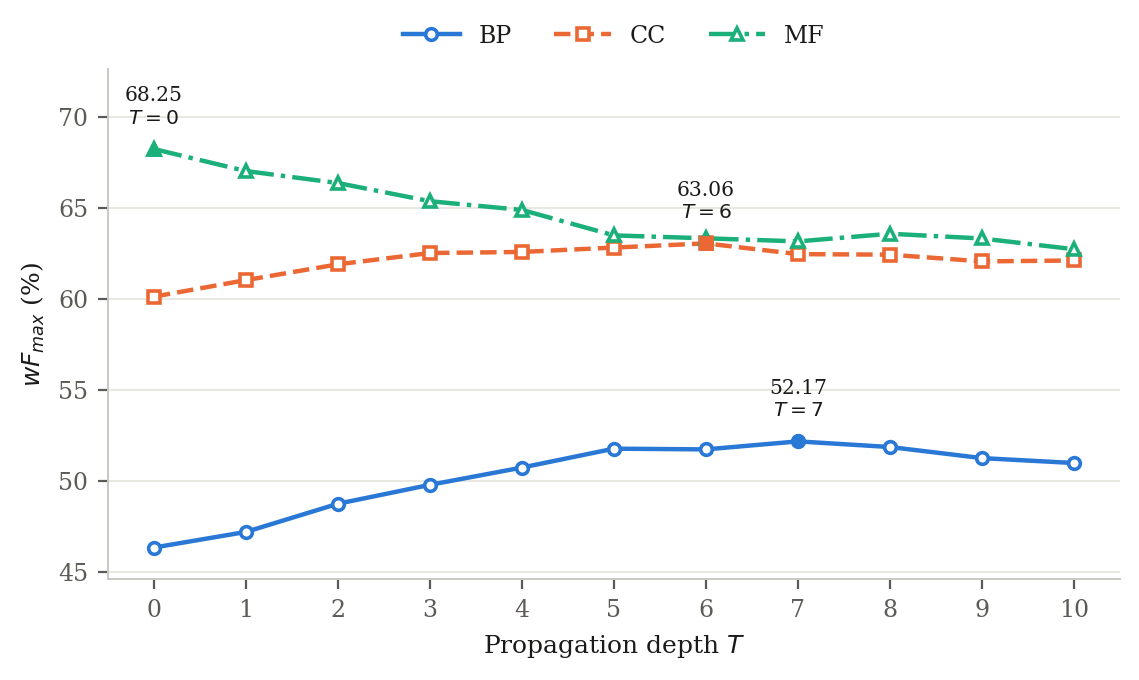
\includegraphics[width=\linewidth]{fig_6_3}
    \column{0.49\textwidth}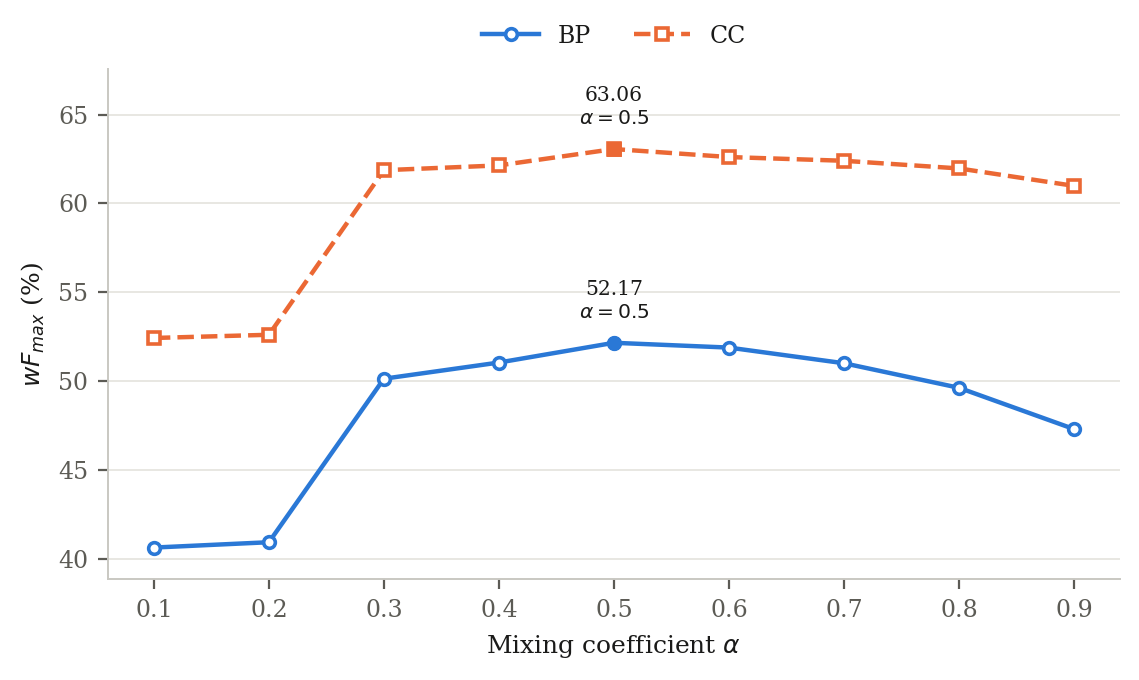
\includegraphics[width=\linewidth]{fig_6_4}
  \end{columns}
  \begin{itemize}
    \item Peak depth: $T=7$ BP, $T=6$ CC, $T=0$ MF; gains over $T=0$: +5.84 BP, +2.93 CC (vector: +1.85, +0.92)
    \item Collapse at $\alpha\le0.2$: isolated nodes shrink as $\alpha^{T}$ ($10^{-7}$ at $T=7$)
    \item Its best BP value, 52.17, is still below the vector head's graph-free 53.36
  \end{itemize}
  \src{Tables 6.7, 6.8; §6.3.1; Figs.~6.3, 6.4}
\end{frame}

\begin{frame}{Learning the aggregation does not pay}
  \begin{center}\small\TabGNN\end{center}
  \begin{itemize}
    \item GCN beats GAT in all 6 pairs (3.88 to 9.31\,pp), and in 30 of 30 fusion pairs
    \item Fixed 65.12 vs GCN 63.32 mean $\wF$: GCN ahead in BP by 0.55 (a tie); behind in CC by 0.59 and MF by 5.35
    \item Deduplication: max never loses beyond noise; GAT gains most (+3.83 vision)
  \end{itemize}
  \src{Tables 6.9, 6.11; §6.3.2, §6.3.3}
\end{frame}

\begin{frame}{Fusion helps; combining predictions helps more}
  \begin{columns}[T]
    \column{0.5\textwidth}
    \resizebox{\linewidth}{!}{\TabLate}\\
    {\scriptsize Late fusion, validation $\wF$ (Table 6.14).}
    \column{0.44\textwidth}
    \begin{itemize}
      \item Early, one configuration (add, GCN, vector): 65.80, +0.68 over fixed alone
      \item Late, linear $\gamma$ (0.50 BP, 0.55 CC and MF): 67.06, best in every ontology
      \item Gains over the better component: +2.18 BP, +1.85 CC, +1.26 MF
      \item Stacking importances: the two probabilities carry almost all the weight
    \end{itemize}
  \end{columns}
  \src{Tables 6.12--6.14; §6.3.4, §6.3.5}
\end{frame}

\begin{frame}{Vector head wins 12 of 12}
  \begin{center}\small\TabVV\end{center}
  \begin{itemize}
    \item Margin on the mean: +6.62, +3.96, +2.69, +3.35\,pp across the four stages; no trend toward zero
    \item Neither image has the locality a convolution assumes
  \end{itemize}
  \src{Tables 6.15, 6.16; §6.4}
\end{frame}

\begin{frame}{Where the gains come from}
  \begin{center}
  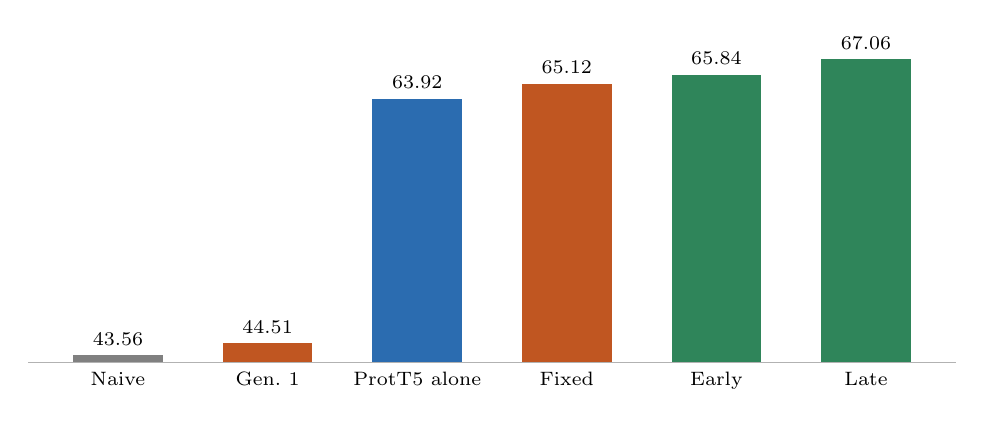
\begin{tikzpicture}[x=1.9cm, y=0.16cm, font=\small]
    \draw[gray!60] (0.4,43) -- (6.6,43);
    \foreach \i/\v/\c/\l in {1/43.56/gray/Naive, 2/44.51/net/Gen.~1, 3/63.92/seq/ProtT5 alone,
                            4/65.12/net/Fixed, 5/65.84/fus/Early, 6/67.06/fus/Late}{
      \fill[\c] (\i-0.3,43) rectangle (\i+0.3,\v);
      \node[above, font=\scriptsize] at (\i,\v) {\v};
      \node[below, font=\scriptsize] at (\i,43) {\l};
    }
  \end{tikzpicture}
  \end{center}
  {\scriptsize Mean validation $\wF$; axis starts at 43. Blue: sequence; orange: network; green: fusion.}
  \begin{itemize}
    \item Most of the jump is the language model; the graph adds the rest
  \end{itemize}
  \src{Tables 6.1, 6.3, 6.5, 6.14, 6.15}
\end{frame}

\begin{frame}{Test set: NEXUS-GO vs five methods (BP)}
  \begin{center}\scriptsize\TabTestBP\end{center}
  \begin{itemize}\small
    \item \NX{Late} best in every column of the three tables, except AuPRC in MF
    \item $\wF$ margin over the strongest baseline: +9.77 BP, +8.67 CC, +4.93 MF
    \item The ProtT5 baseline alone already beats every literature method on $\wF$
  \end{itemize}
  \src{Tables 6.17--6.19; §6.5; Appendix B (CC and MF in backup)}
\end{frame}

\begin{frame}{Every protein gets a prediction}
  \begin{center}\small\TabCov\end{center}
  \begin{itemize}
    \item DeepGraphGO and SEGT-GO reach unseen proteins through homology search
    \item Mashup, MELISSA, deepNF score only network members; missing proteins count as misses
    \item Part of the distance to network-only methods is reach, not ranking quality
  \end{itemize}
  \src{Table 6.28; Table B.3}
\end{frame}

\begin{frame}{A thirteenth of the time per epoch}
  \begin{columns}[c]
    \column{0.5\textwidth}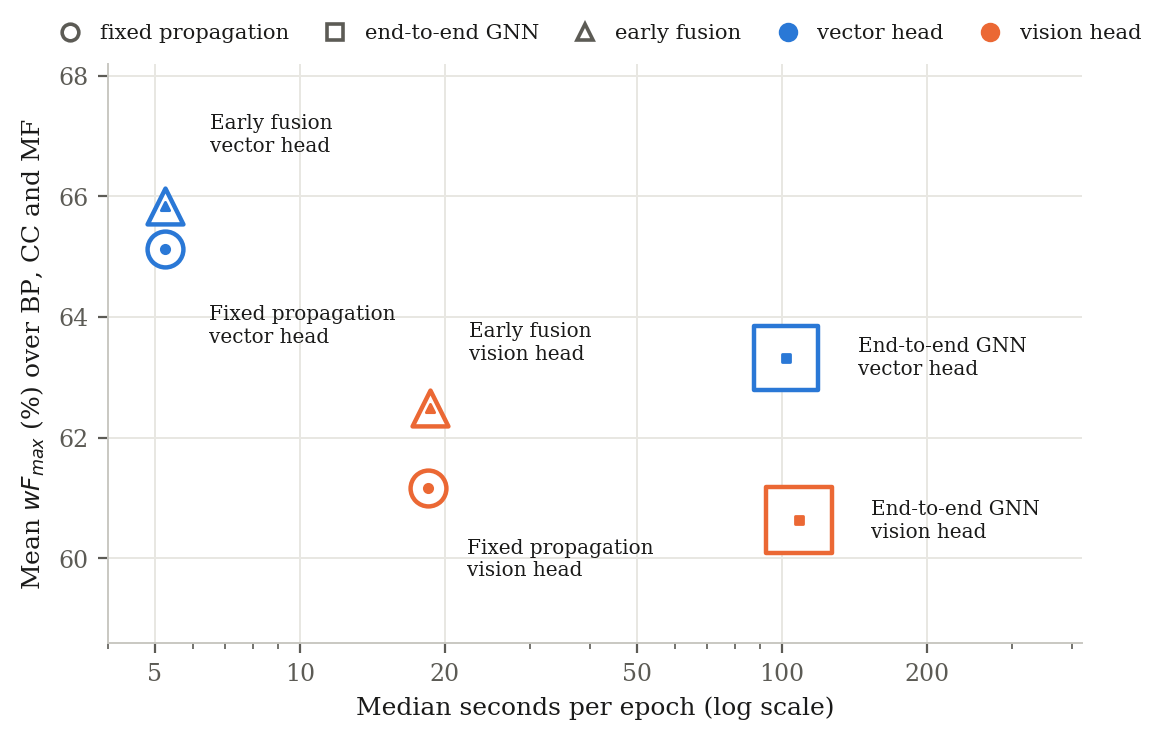
\includegraphics[width=\linewidth]{fig_6_5}
    \column{0.48\textwidth}
    \begin{itemize}
      \item Fixed + vector: 5.24\,s/epoch, 6.4\,GiB peak
      \item GCN alone: 68.76\,s/epoch, 14.1\,GiB; GAT 161.41\,s, 20.7\,GiB
      \item \alert{Matches or beats the GCN at about 1/13 of the time and under half the memory}
      \item Early fusion costs the same as fixed propagation once $g$ is stored
    \end{itemize}
  \end{columns}
  \src{Table 6.20; §6.6.1; Appendix A.7; Fig.~6.5}
\end{frame}

\begin{frame}{The graph helps where there is graph}
  \begin{columns}[c]
    \column{0.56\textwidth}
    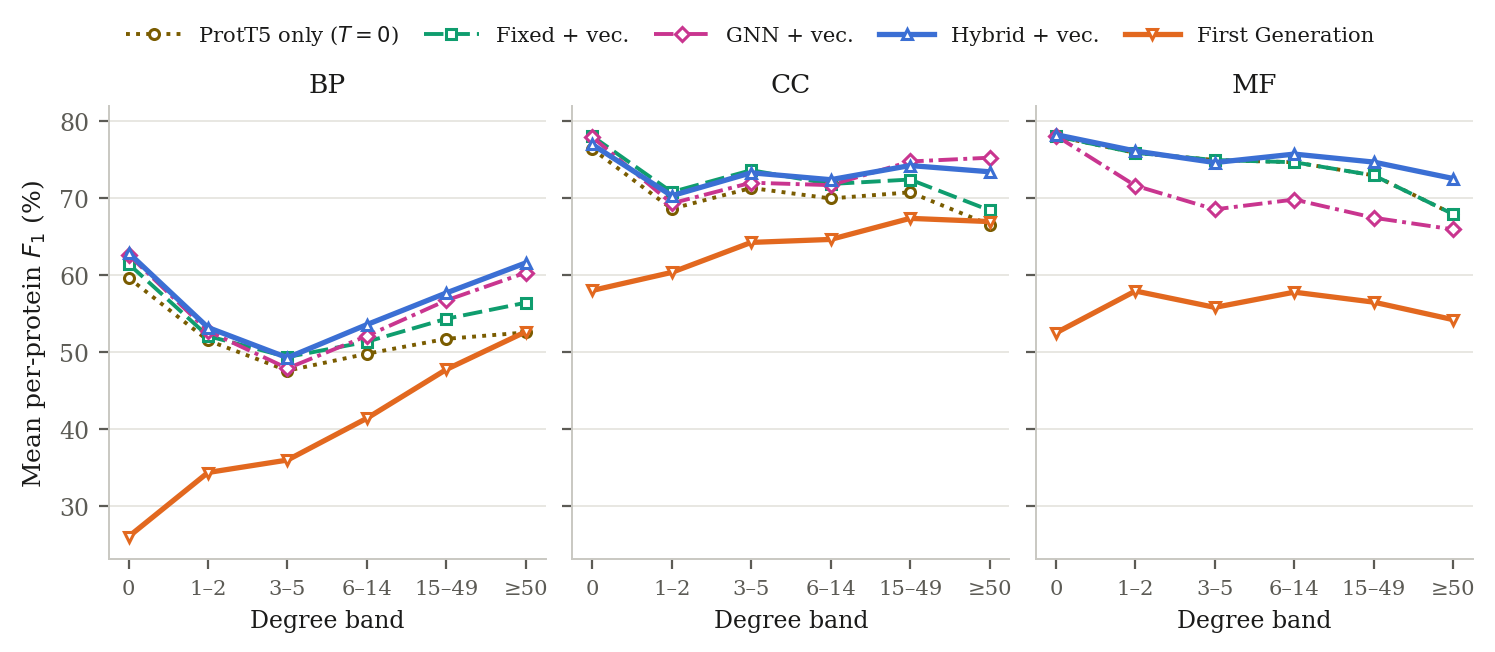
\includegraphics[height=0.32\textheight]{fig_6_6}\\[0.2em]
    \centering{\scriptsize\TabGain}\\
    {\scriptsize Gain over the $T=0$ control, per-protein $F_1$, test, pp; f fixed, g GNN, h early fusion.}
    \column{0.42\textwidth}
    \begin{itemize}
      \item Every ProtT5 route scores worse on connected than on isolated proteins
      \item The graph-free control already shows it, so the graph does not cause it
      \item The graph's gain grows with degree: up to +9.05 BP, +8.71 CC, +4.64 MF at degree $\ge 50$
    \end{itemize}
  \end{columns}
  \src{Tables 6.21--6.27; Fig.~6.6; §6.6.2}
\end{frame}

% ============================================================================ Conclusions
\section{Conclusions}

\begin{frame}{Answers to the research questions}
  \small
  \begin{description}[RQ7]
    \item[RQ1] The unreduced profile and an MLP; imposed locality hurts
    \item[RQ2] Large gain, mostly from ProtT5; propagation adds +1.87 BP, +2.15 CC, nothing in MF (test)
    \item[RQ3] Late 67.06 $>$ Early 65.84 $>$ Fixed 65.12 $>$ GNN 63.32 (validation); vector head throughout
    \item[RQ4] Both help; late more (+1.26 to +2.18\,pp, validation)
    \item[RQ5] One or two hops, $\alpha$ 0.7--0.8; MF prefers none
    \item[RQ6] Best in every column but one; +9.77 / +8.67 / +4.93\,pp $\wF$ (test)
    \item[RQ7] Works on one global aggregated network; partitioned graphs not tested
  \end{description}
  \src{Chapter 7}
\end{frame}

\begin{frame}{Limitations}
  \begin{itemize}
    \item Single seed; the 0.5\,pp floor is a reading convention, not a confidence interval
    \item Random protein-level split: transductive interpolation, possible homology leakage
    \item STRING scores may encode annotation knowledge (circularity)
    \item Fixed vs learned is not a single-factor ablation ($\alpha^{T}$ scaling, normalization)
    \item Baselines adapted to one aggregated network and a reduced label space
  \end{itemize}
  \src{Chapter 7}
\end{frame}

\begin{frame}{Next steps}
  \begin{itemize}
    \item Separate the graph by organism, or one model per organism
    \item Keep STRING evidence channels apart (typed or parallel edges)
    \item Heterogeneous graphs (proteins, terms, evidence); compare with ProtHGT
    \item Sampled aggregation (GraphSAGE) for a cheaper learned route
    \item Richer node features: structure, domains, expression; most promising for MF
  \end{itemize}
  \src{Chapter 7}
\end{frame}

\begin{frame}{Thank you}
  \begin{itemize}
    \item NEXUS-GO: fixed propagation of ProtT5 over STRING, fused with a GCN, best in every ontology at a fraction of the cost
    \item Code: \texttt{github.com/ymauhn/nexus-go}
    \item Publications: VISAPP 2026; extended version accepted in CCIS (expected December 2026)
    \item Funding: CAPES, BTG Pactual \,·\, Computing resources: IC/Unicamp
  \end{itemize}
  \vspace{1.5em}
  \centering{\Large\color{ink}Questions}
\end{frame}

% ============================================================================ Backup
\appendix
\section*{Backup}

\begin{frame}{Backup: test set, Cellular Component (CC)}
  \begin{center}\scriptsize\TabTestCC\end{center}
  \src{Table 6.18}
\end{frame}

\begin{frame}{Backup: test set, Molecular Function (MF)}
  \begin{center}\scriptsize\TabTestMF\end{center}
  \src{Table 6.19}
\end{frame}

\begin{frame}{Backup: computational cost by family}
  \begin{center}\scriptsize\TabCost\end{center}
  {\scriptsize RTX A5500, 147 runs; lowest value in bold for s/epoch, h/run and VRAM.}
  \src{Table 6.20}
\end{frame}

\end{document}
